%%%%%%%%%%%%%%
% Evaluation %
%%%%%%%%%%%%%%

\chapter{Evaluation}
\label{chapter:evaluation}

Den Gegenstand dieses Kapitels bildet eine Evaluation des umgesetzten Konzepts, die aus zwei Teilen besteht. Zum einen basiert sie auf einer Nutzerstudie, deren Beschreibung und Auswertung sich der Abschnitt \ref{sec:user-study} widmet. Zum anderen wird in Abschnitt \ref{sec:criteria-evaluation} gezeigt, dass die für das Konzept aufgestellten Kriterien eingehalten wurden. Das Kapitel schließt mit einer Zusammenfassung in Abschnitt \ref{sec:evaluation-summary}.

\section{Nutzerstudie}
\label{sec:user-study}

Um das Konzept an reellen Nutzern zu validieren, wurde im Rahmen der Bachelor-Arbeit eine Nutzerstudie durchgeführt, die im Folgenden erläutert wird. Zunächst werden in Abschnitt \ref{subsec:user-study-setup} der Aufbau und die Durchführung im Detail beschrieben. Anschließend folgt in Abschnitt \ref{subsec:user-study-evaluation} eine Auswertung der Ergebnisse.

\subsection{Aufbau und Durchführung}
\label{subsec:user-study-setup}

Die Nutzerstudie wurde in individuelle Sitzungen aufgeteilt. Jede Sitzung hat mit einer kurzen Beschreibung des Themas der Bachelor-Arbeit angefangen. Danach wurde der Ablauf der Sitzung vorgestellt und der Teilnehmer wurde um das Ausfüllen des ersten Teils des vorgefertigten Fragebogens (siehe Abschnitt \ref{sec:user-study-material-questionnaire}) gebeten, in dem allgemeine Informationen und Vorkenntnisse abgefragt wurden. Nach Bedarf wurde anschließend eine kurze Einführung über Klassendiagramme gegeben, um die Notation und die wichtigsten Begriffe wie Klasse, Vererbung, Oberklasse und Unterklasse zu erklären.

Die eigentlichen Tests des entwickelten Prototyps (siehe Kapitel \ref{chapter:prototype}) wurden an einem \textit{MacBook Pro} durchgeführt. Als Eingabegerät stand den Teilnehmern das in dem Notebook eingebaute Trackpad, eine \textit{Apple Magic Mouse}\footnote{\url{https://www.apple.com/magicmouse}} und eine klassische optische Maus zur Verfügung. Um potenzielle Probleme mit der Eingabe zu vermeiden, konnten die Teilnehmer frei das passende Eingabegerät wählen.

Als Nächstes wurde eine kurze Einführung zu dem Prototyp gegeben. Die unterstützten Aktionen wie das Erstellen bzw. Umbenennen einer Klasse, Erstellen einer Vererbungsrelation und Löschen des Diagramms wurden beschrieben und im Prototyp demonstriert. Insbesondere wurden die zwei Möglichkeiten zum Erstellen der Vererbungsrelation gezeigt, nämlich durch das Anklicken des Icons in der Sidebar und durch das Drücken der der Taste \texttt{CTRL} (siehe Abschnitt \ref{subsec:supported-actions}). Nach dieser Einführung durfte der Teilnehmer den Prototyp für ca. zwei Minuten ausprobieren.

Der eigentliche Test bestand darin, vier verschiedene Aufgaben zur Modellierung von Klassendiagrammen mit Vererbungshierarchien zu erfüllen. Alle Aufgaben haben das baumbasierte Layout benötigt, so dass die Lay\-out-Engine nicht geändert werden musste. Dem Teilnehmer wurden nacheinander Blätter mit den Aufgabenstellungen vorgelegt, die durch ihn gelöst wurden. Zum einen handelte sich um visuelle Aufgaben, in den der Teilnehmer ein bestehendes Diagramm rekonstruieren sollte. Zum anderen hatten die Aufgaben die Form einer textuellen Beschreibung. Alle Aufgabenblätter sind im Anhang unter Abschnitt \ref{sec:user-study-material-task-description} abgebildet.

Die Teilnehmer wurden gebeten, während der Erfüllung der Aufgaben ihr Vorgehen laut zu beschreiben. Dabei wurden die wichtigsten Beobachtungen notiert. Weiterhin wurde der Bildschirm aufgenommen, um eventuelle weitere Analysen zu ermöglichen. Die Videodateien sind auf der beigelegten DVD zu finden (für das Dateienverzeichnis siehe Abschnitt \ref{sec:files-user-study}).

Im Anschluss wurde das Konzept durch den Teilnehmer bewertet, indem der verbleibende Teil des Fragebogens (siehe Abschnitt \ref{sec:user-study-material-questionnaire}) ausgefüllt wurde. Obwohl die Teilnehmer in den letzten Fragen des Fragebogens eine Möglichkeit hatten, ein allgemeines Feedback zu geben, wurde in einzelnen Fällen eine Diskussion bevorzugt.

\subsection{Auswertung}
\label{subsec:user-study-evaluation}

An der Nutzerstudie haben insgesamt 7 Testpersonen teilgenommen und beide Geschlechter wurden ungefähr gleichmäßig vertreten (4 männliche und 3 weibliche Teilnehmer). Großteils handelte sich um Studenten und wissenschaftliche Arbeiter zwischen 21 und 34 Jahren. Des Weiteren waren 6 von 7 Teilnehmern im Bereich der Informatik tätig und waren daher mit der Notation von Klassendiagrammen vertraut.

Vor dem Test wurden die Teilnehmer in dem Fragebogen (siehe Abschnitt \ref{sec:user-study-material-questionnaire}) befragt, welche Werkzeuge sie zum Erstellen von Diagrammen benutzen und in welchen Maß. Die kompletten Ergebnisse sind in Form von Diagrammen in Abbildung \ref{fig:used-tools-charts} veranschaulicht. Es stellt sich heraus, dass die Teilnehmer Stift und Papier zum Zeichnen von Diagrammen am häufigsten verwenden. Das kann dadurch begründet werden, dass dies oft die einfachste Methode ist \cite{Ambler02Agile}. Die Softwarewerkzeuge werden in kleinerem Maß eingesetzt, dennoch ist deren Nutzung nicht vernachlässigbar. Überwiegend werden die Diagramme in Präsentationsprogrammen gezeichnet, es werden aber auch Diagramm-Programme und UML-Editoren zum Einsatz gebracht. Dagegen sind die Ergebnisse der Nutzung von Online-Tools eher gering. 

\begin{figure}[hbt]
\newcommand{\legendscale}{0.9}
\newcommand{\subfigurewidth}{0.3\linewidth}
\newcommand{\graphicsscale}{0.75}    
\centering
\begin{minipage}{.15\textwidth}
    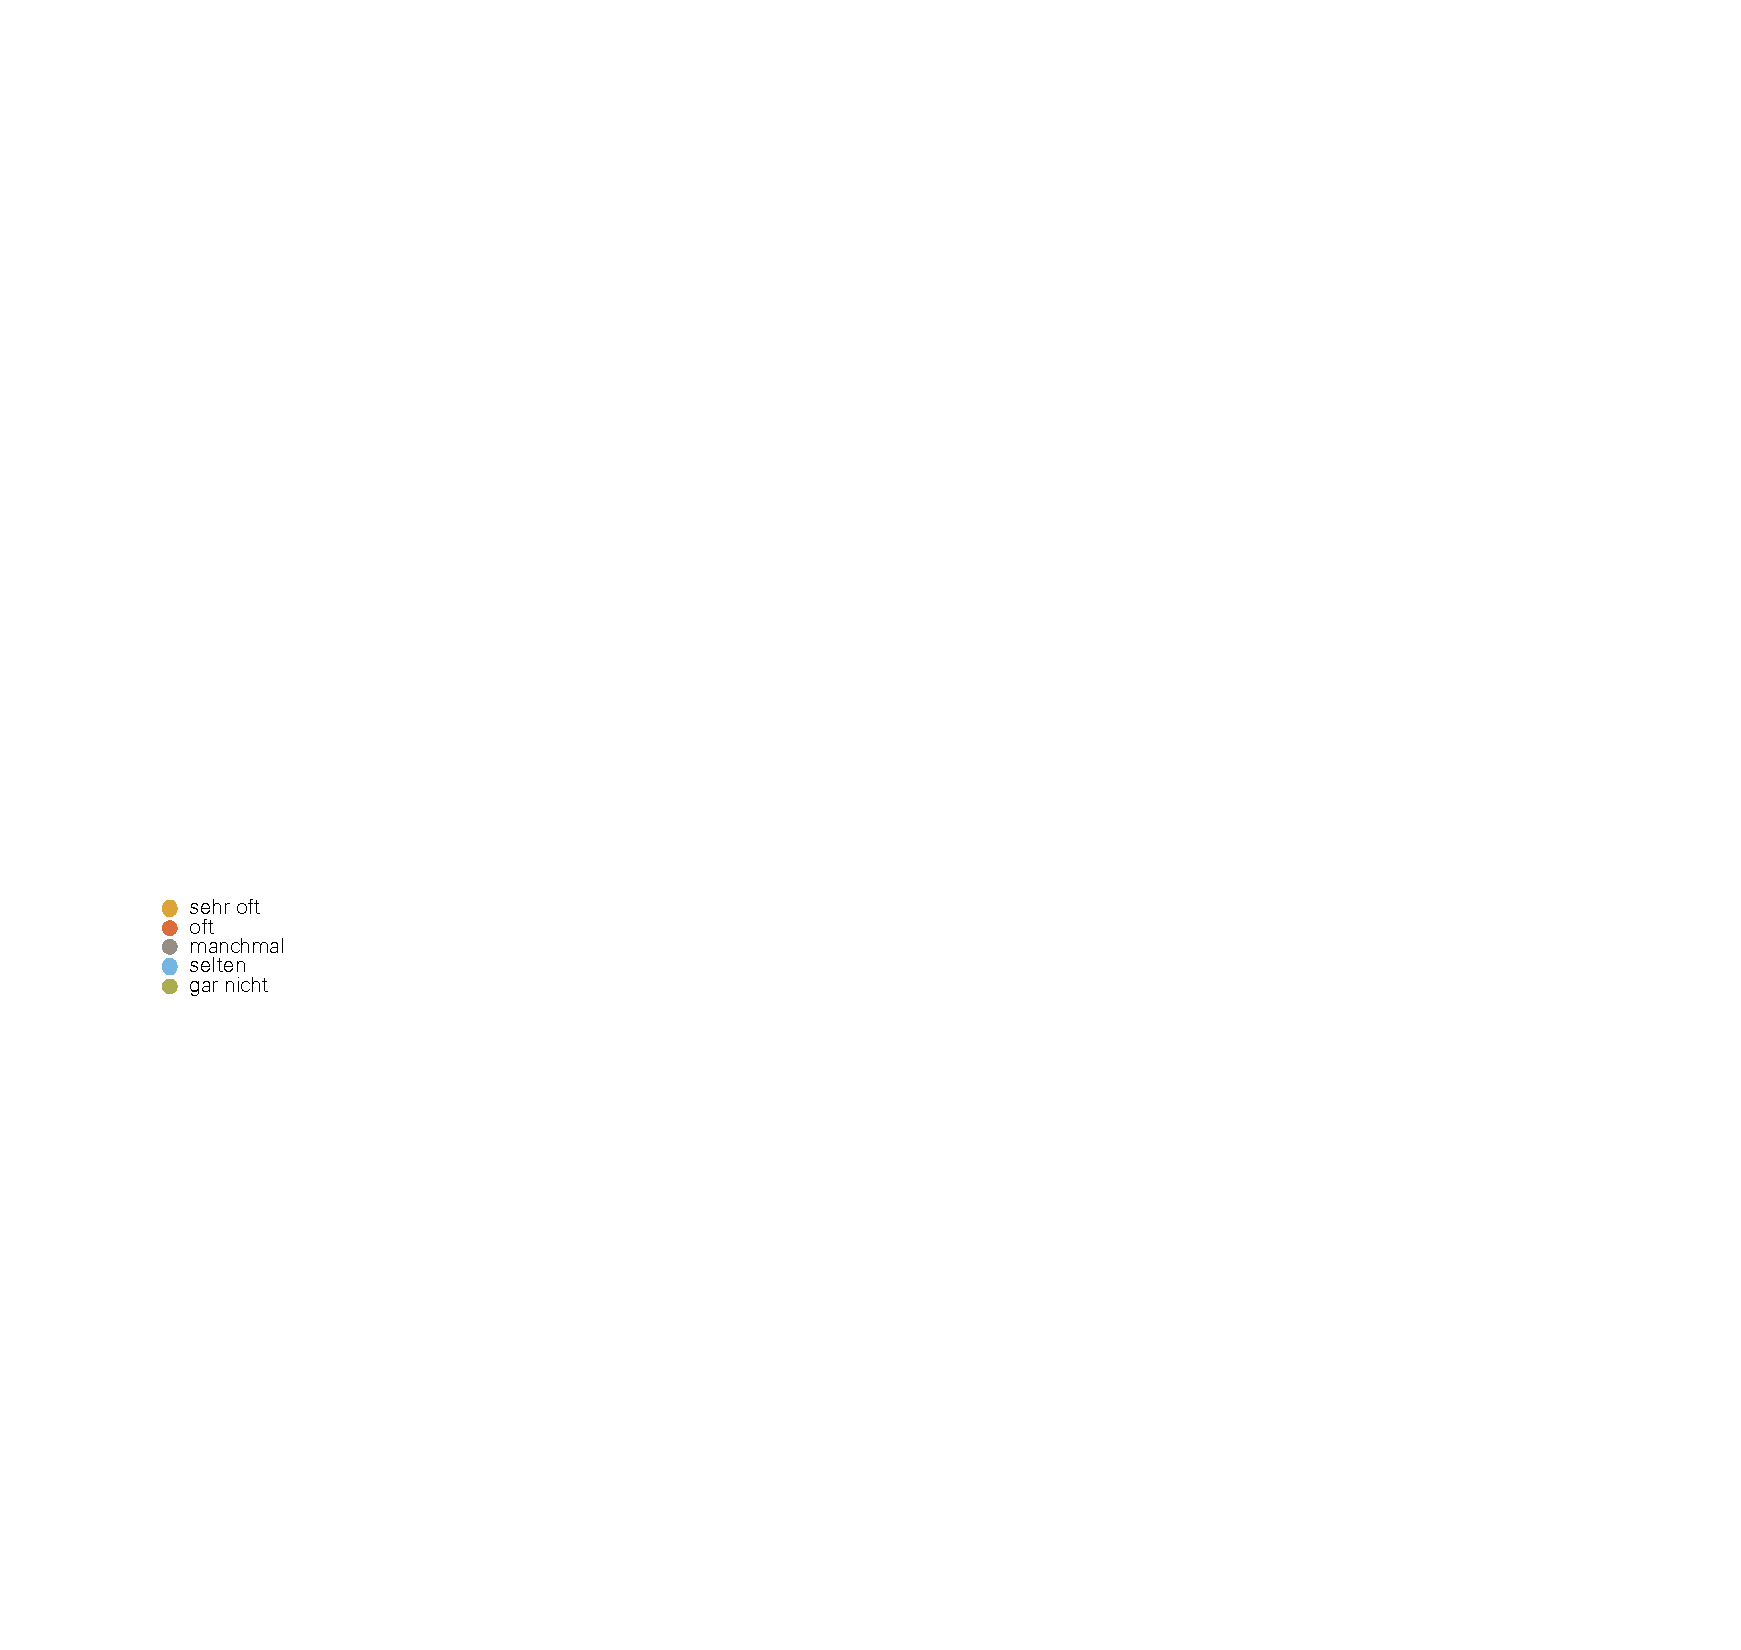
\includegraphics[scale=\legendscale]{resources/used-tools-charts-legend}
\end{minipage}
\begin{minipage}{.65\textwidth}
    \centering
    \begin{subfigure}[t]{\subfigurewidth}
        \centering
        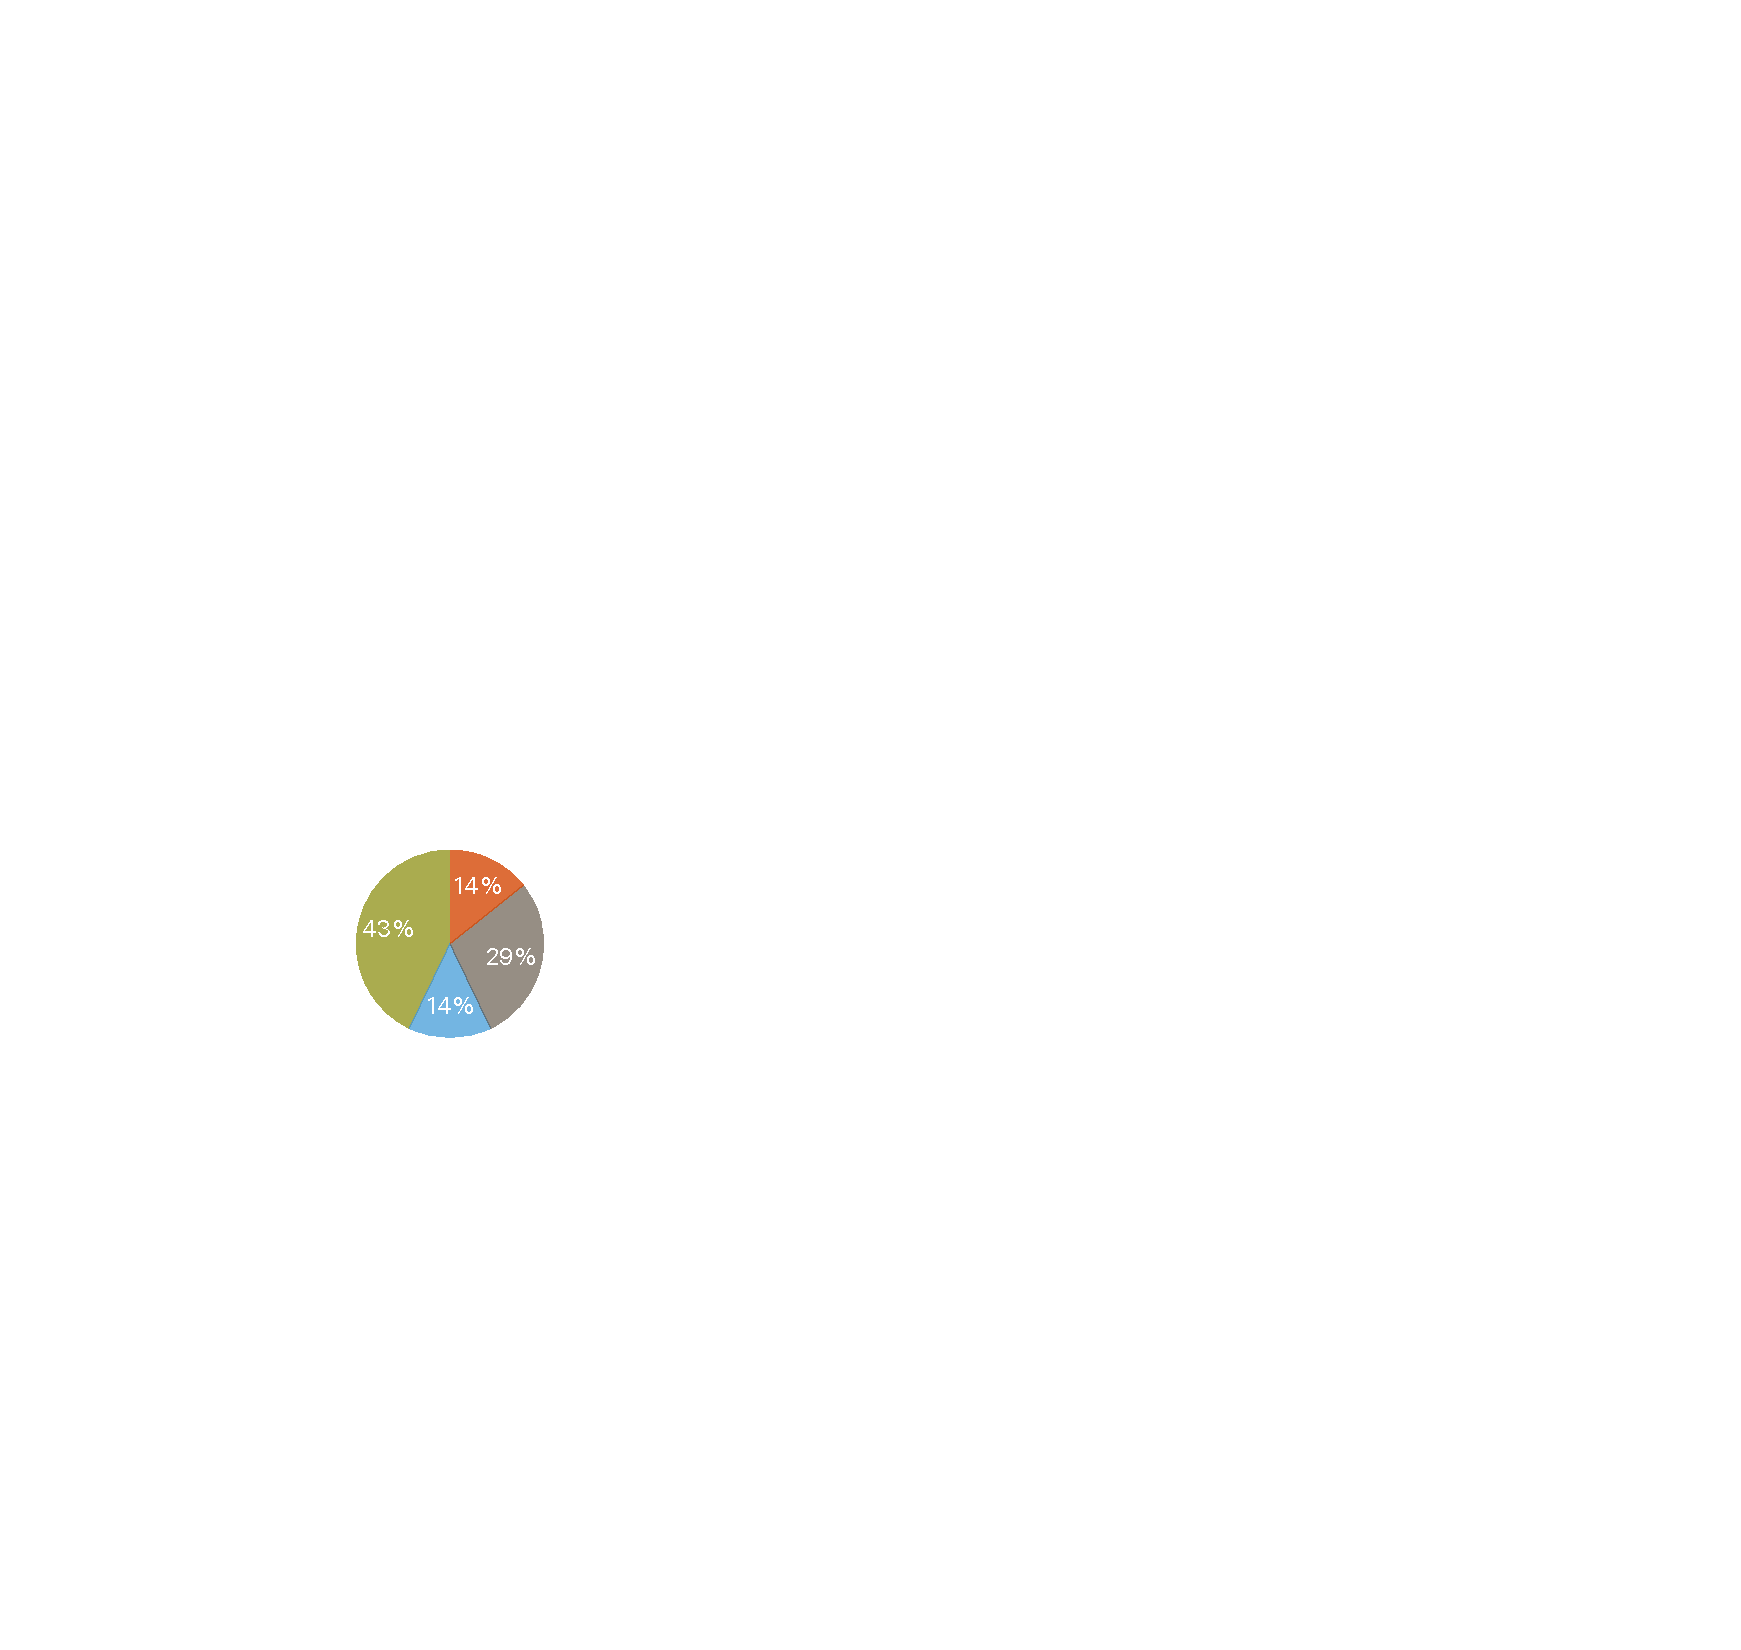
\includegraphics[scale=\graphicsscale]{resources/used-tools-charts-a}
        \caption{Diagramm-Programme}
        \label{fig:used-tools-charts-a}
    \end{subfigure}
    \begin{subfigure}[t]{\subfigurewidth}
        \centering
        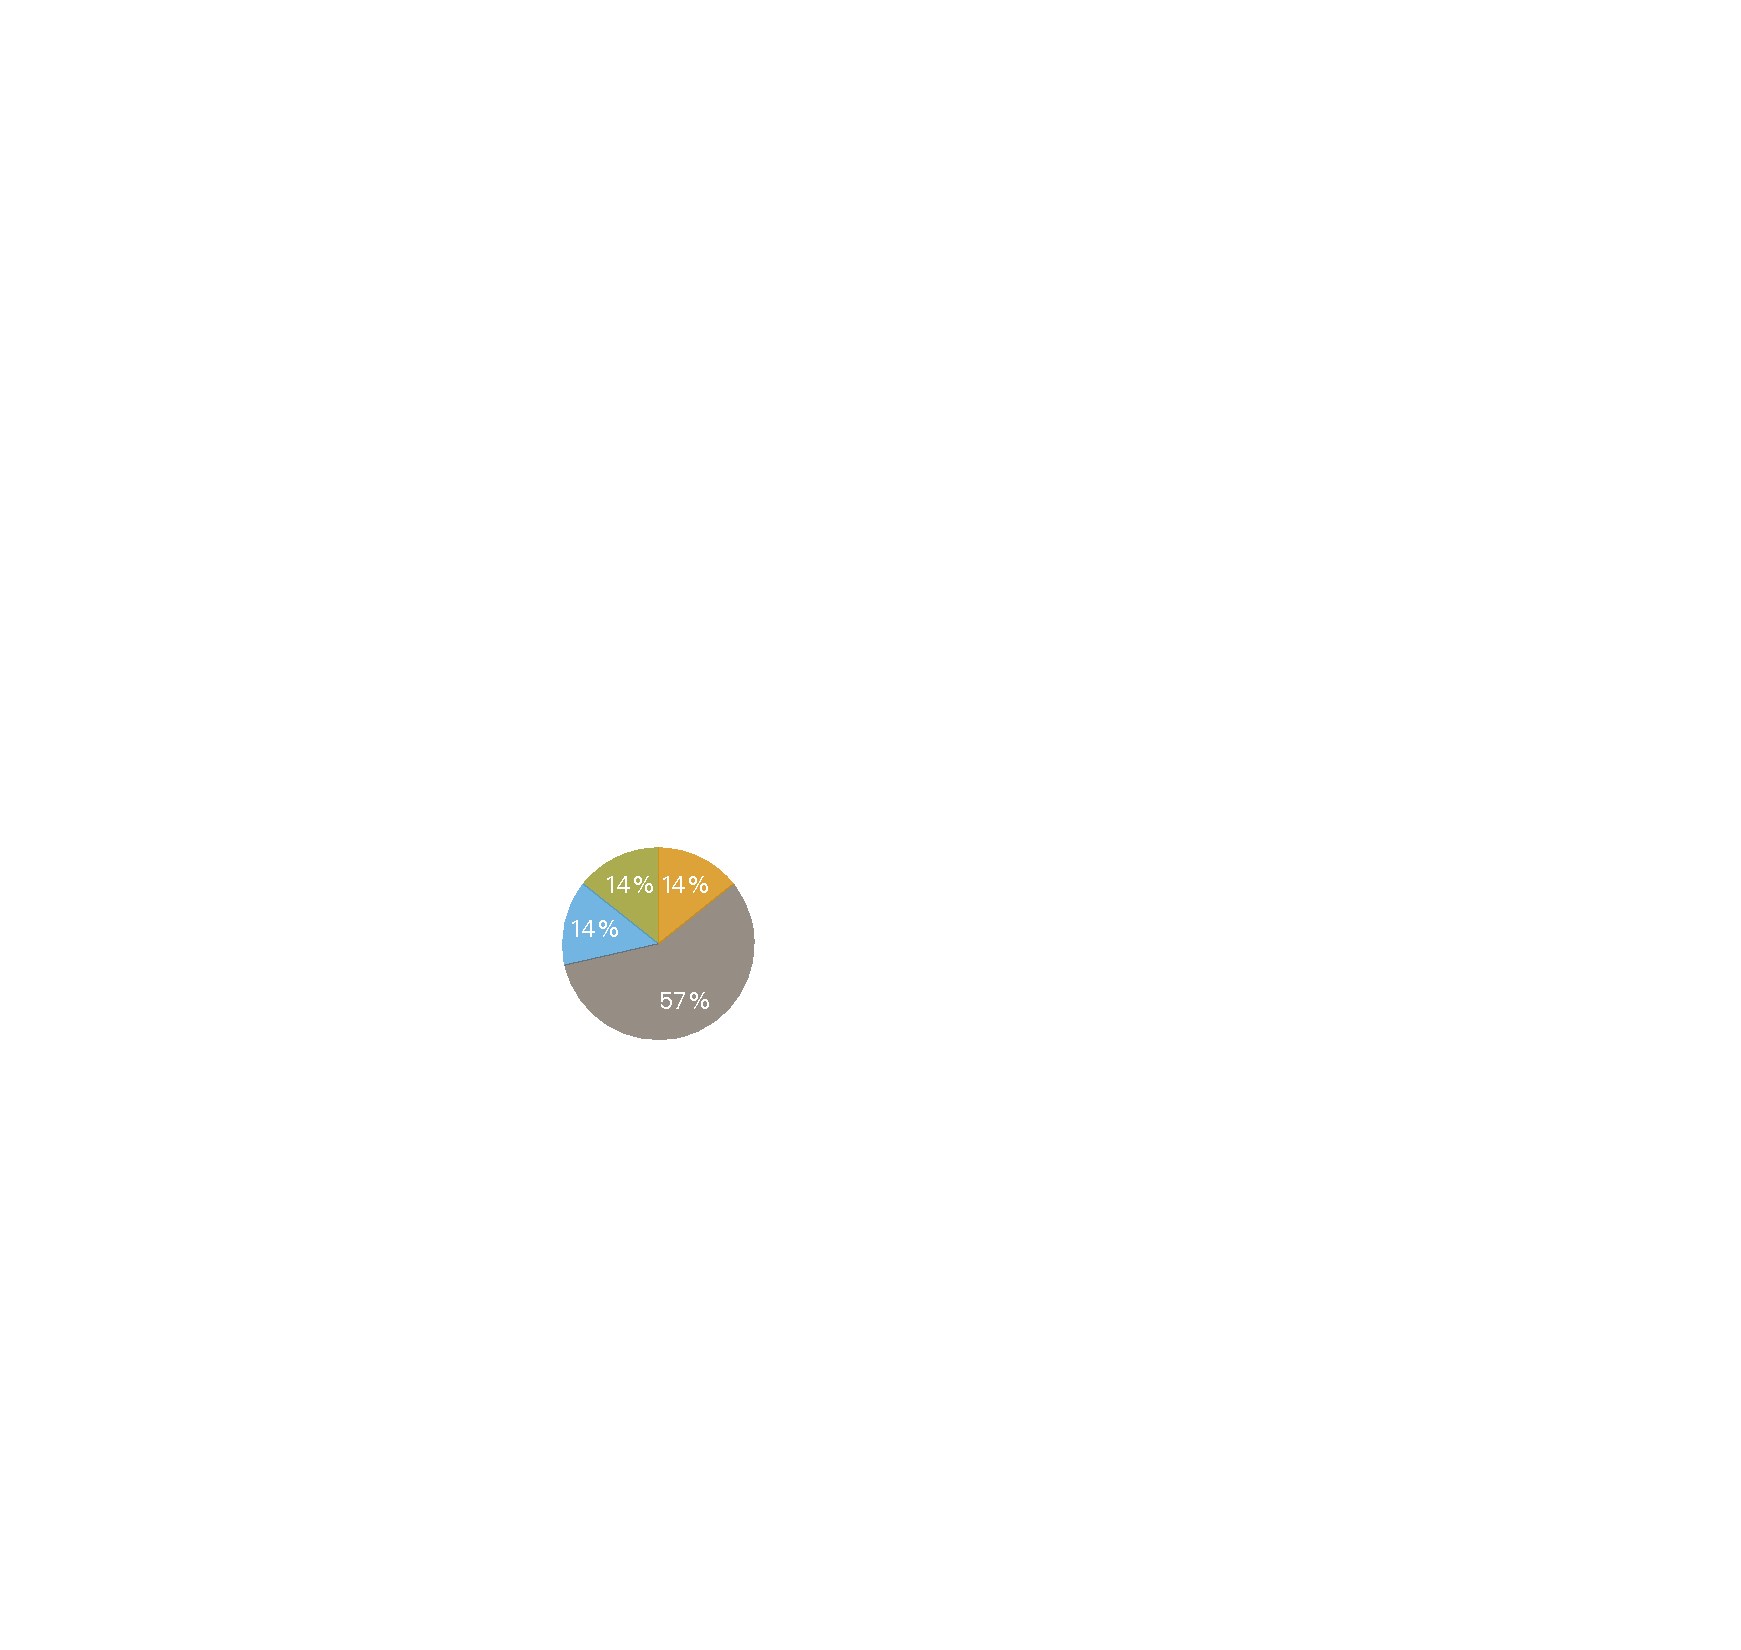
\includegraphics[scale=\graphicsscale]{resources/used-tools-charts-b}
        \caption{Präsentationsprogramme}
        \label{fig:used-tools-charts-b}
    \end{subfigure}
    \begin{subfigure}[t]{\subfigurewidth}
        \centering
        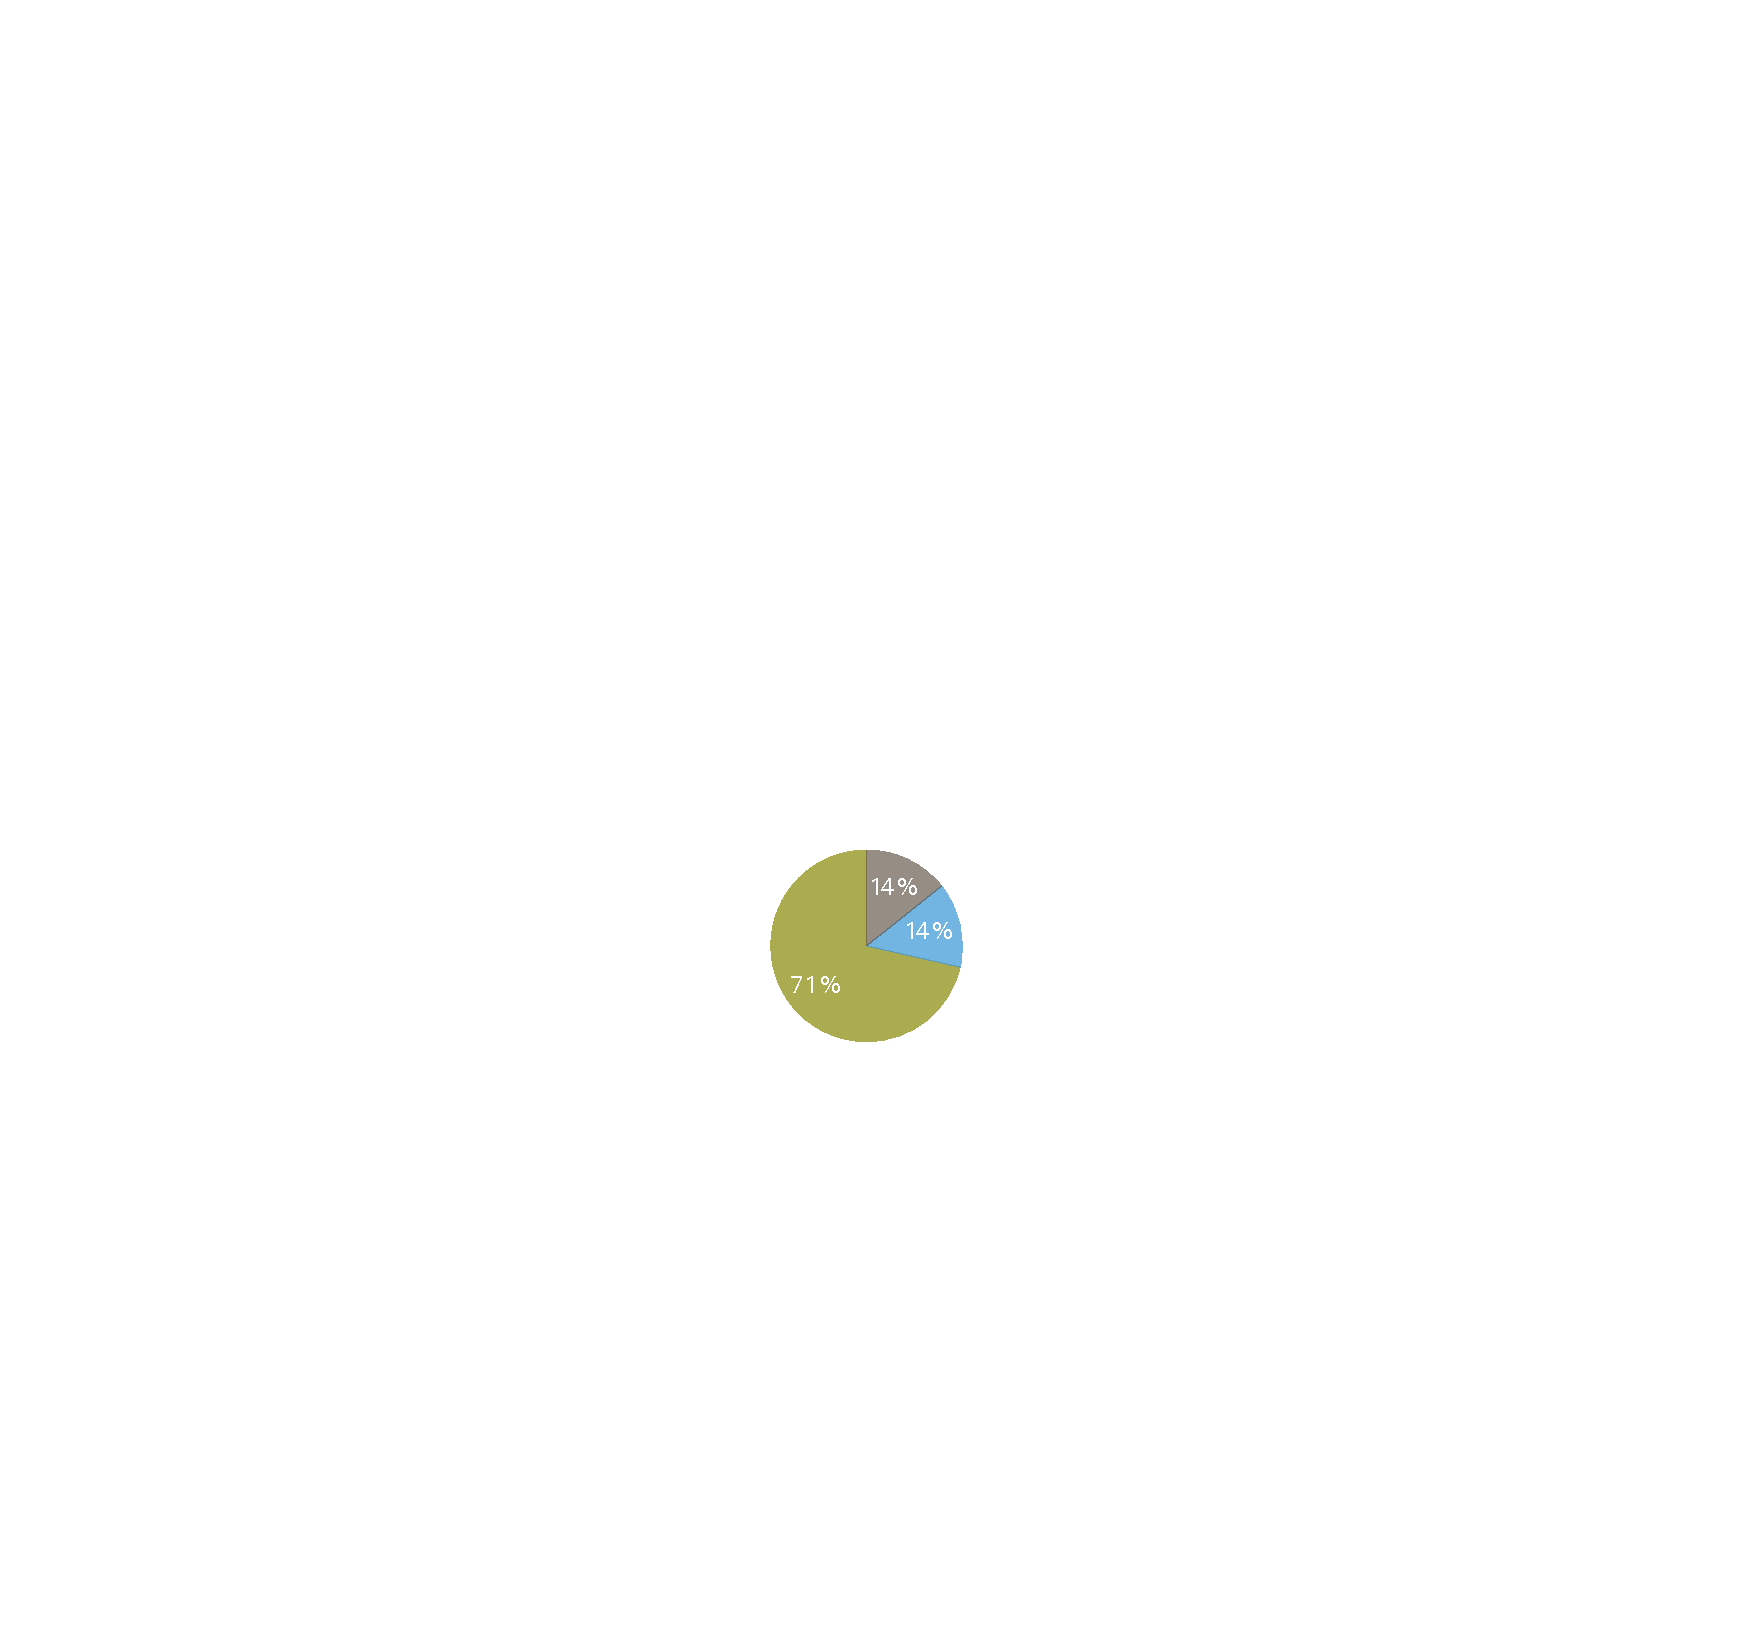
\includegraphics[scale=\graphicsscale]{resources/used-tools-charts-c}
        \caption{Online-Tools}
        \label{fig:used-tools-charts-c}
    \end{subfigure}
    \begin{subfigure}[t]{\subfigurewidth}
        \centering
        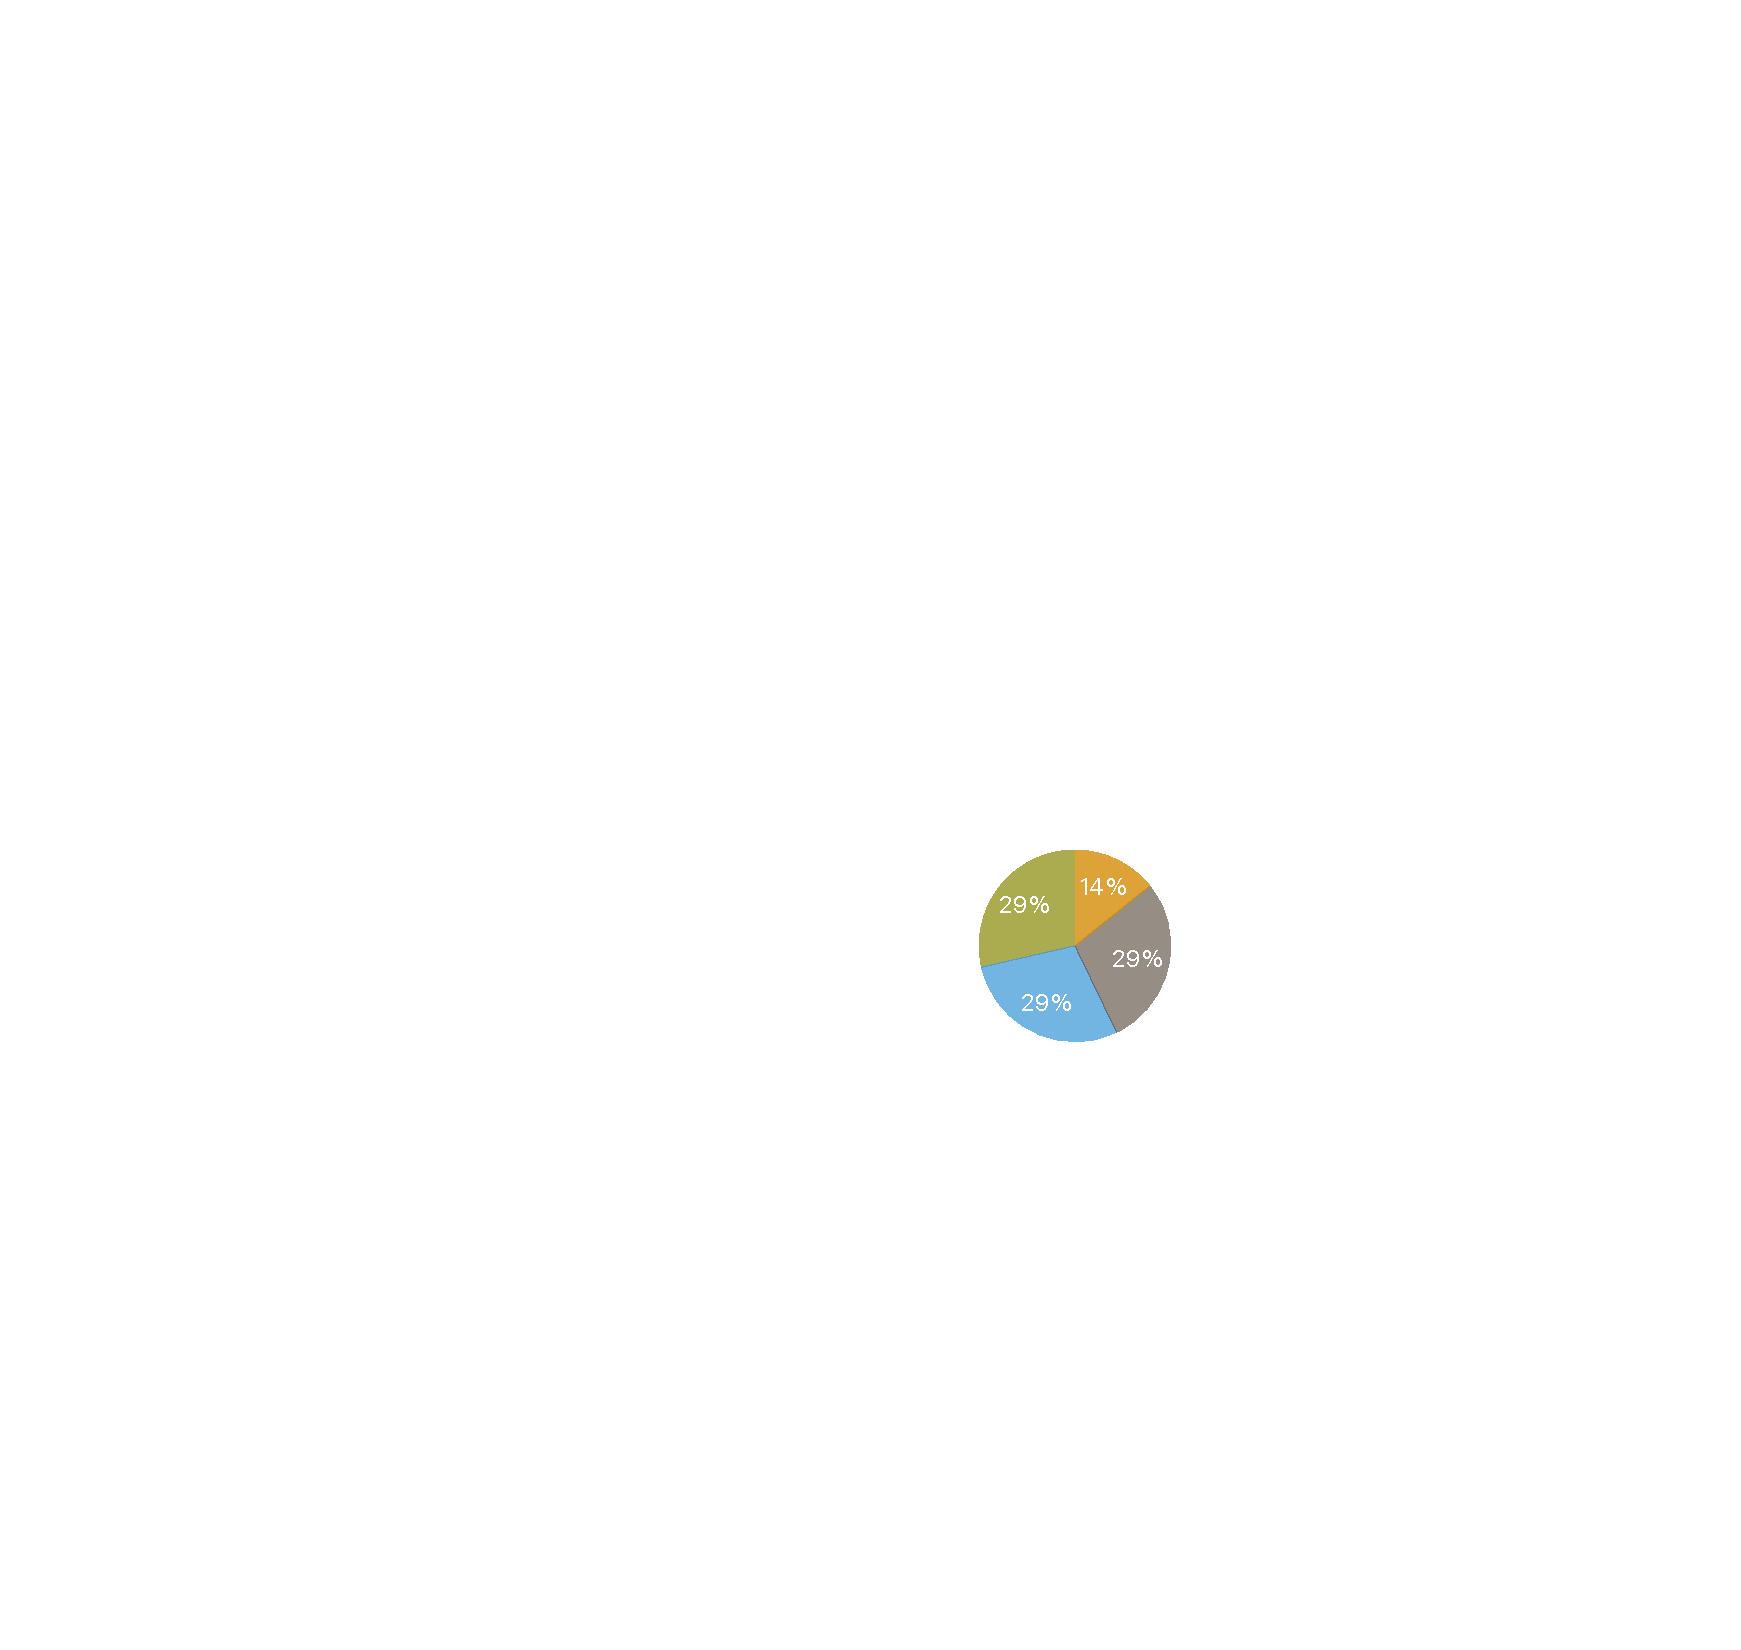
\includegraphics[scale=\graphicsscale]{resources/used-tools-charts-d}
        \caption{UML-Editoren}
        \label{fig:used-tools-charts-d}
    \end{subfigure}
    \begin{subfigure}[t]{\subfigurewidth}
        \centering
        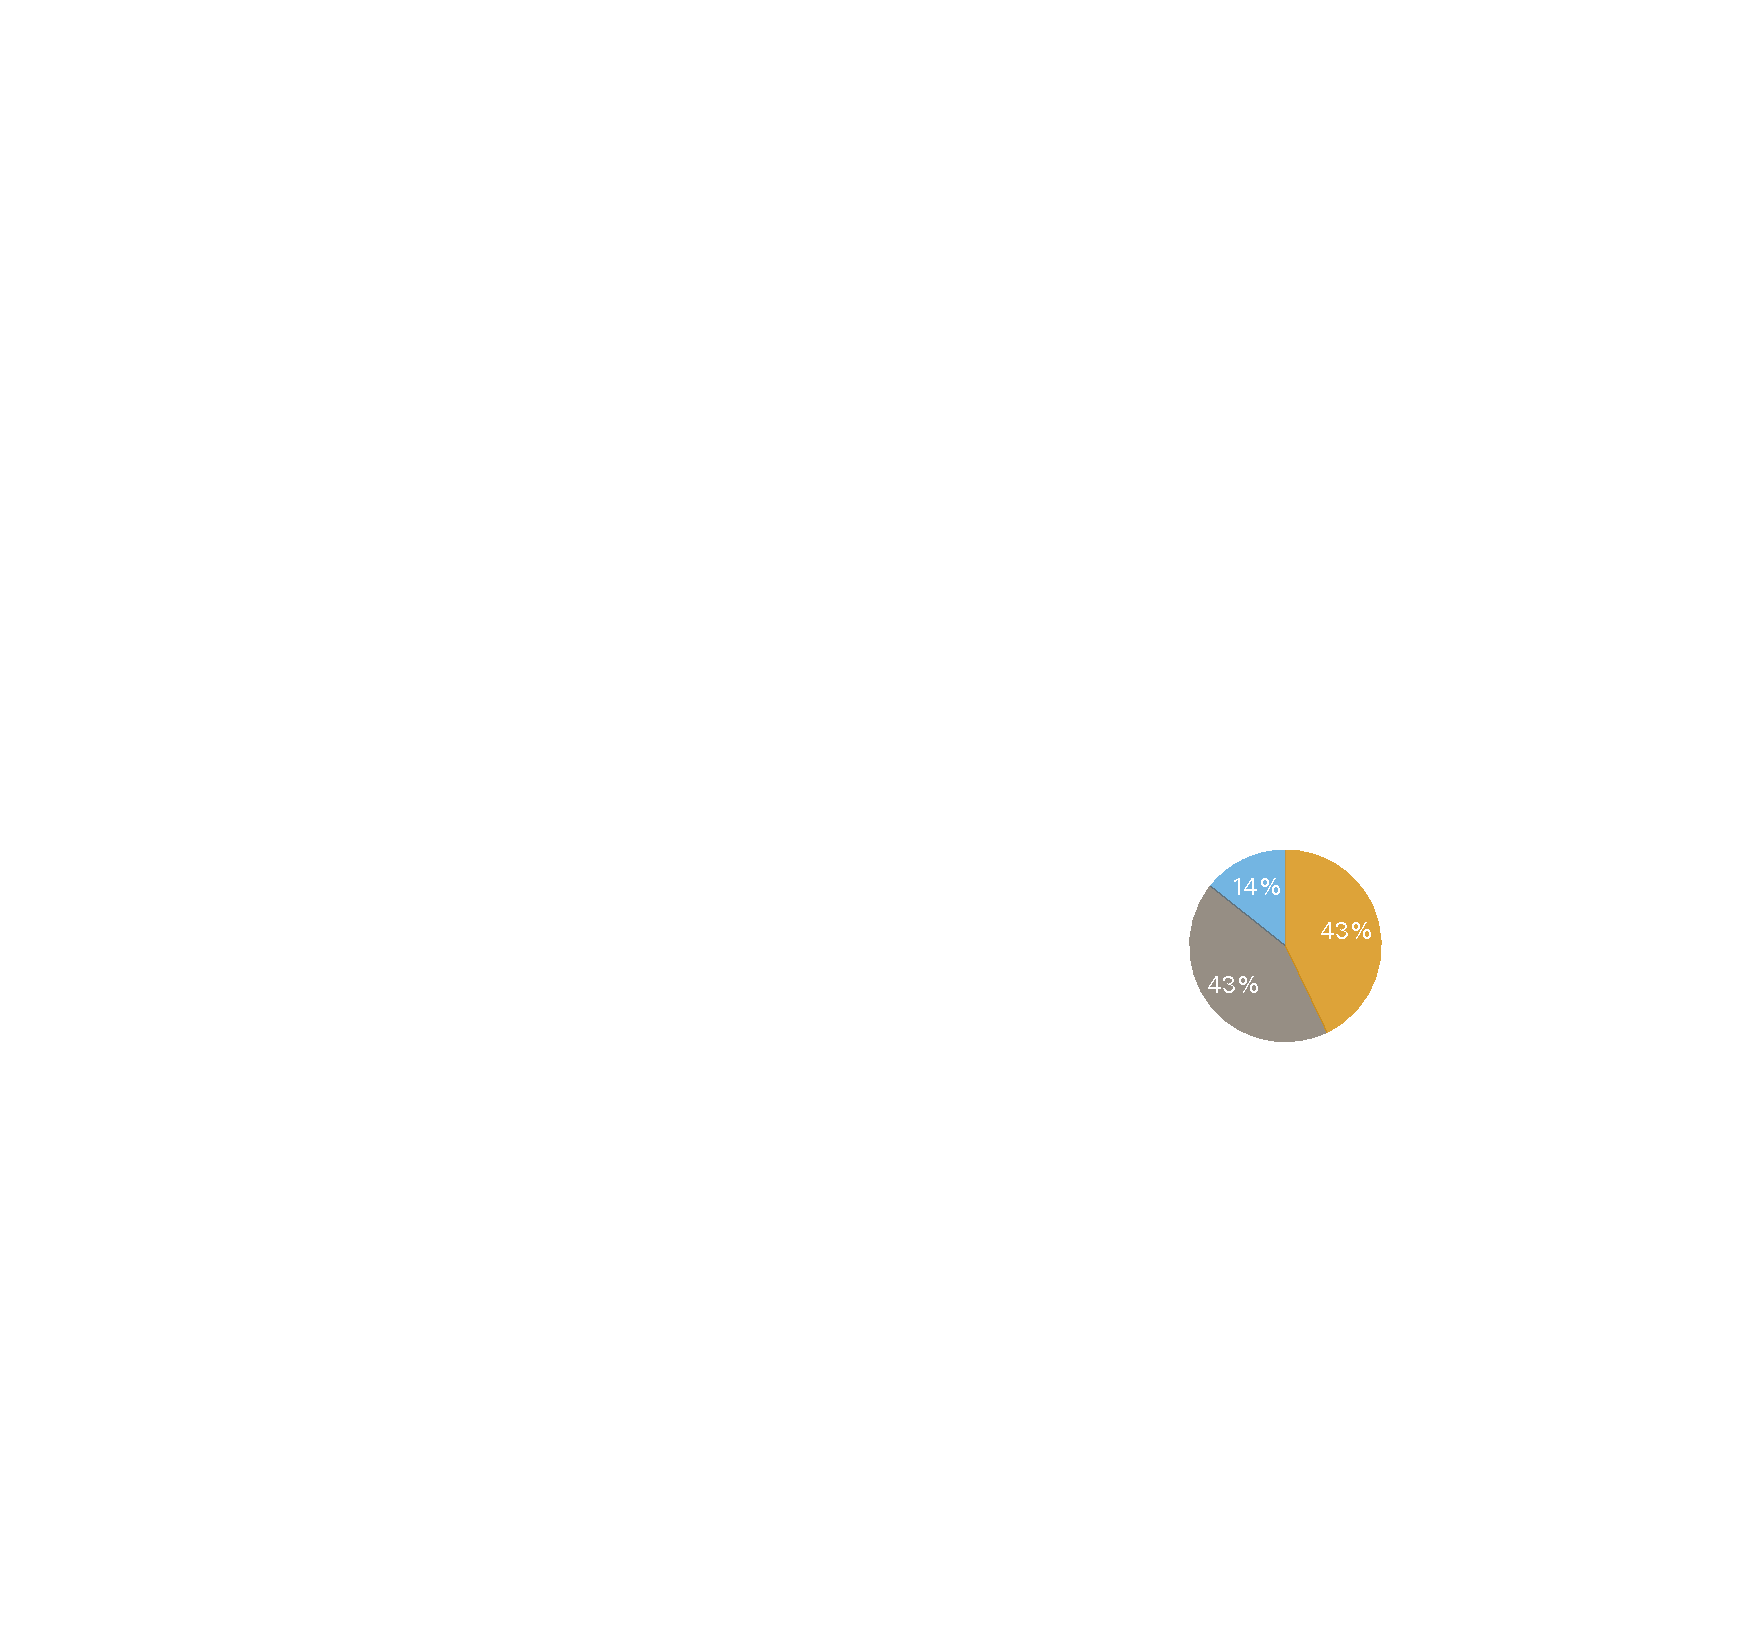
\includegraphics[scale=\graphicsscale]{resources/used-tools-charts-e}
        \caption{Stift und Papier}
        \label{fig:used-tools-charts-e}
    \end{subfigure}
    \begin{subfigure}[t]{\subfigurewidth}
        \centering
        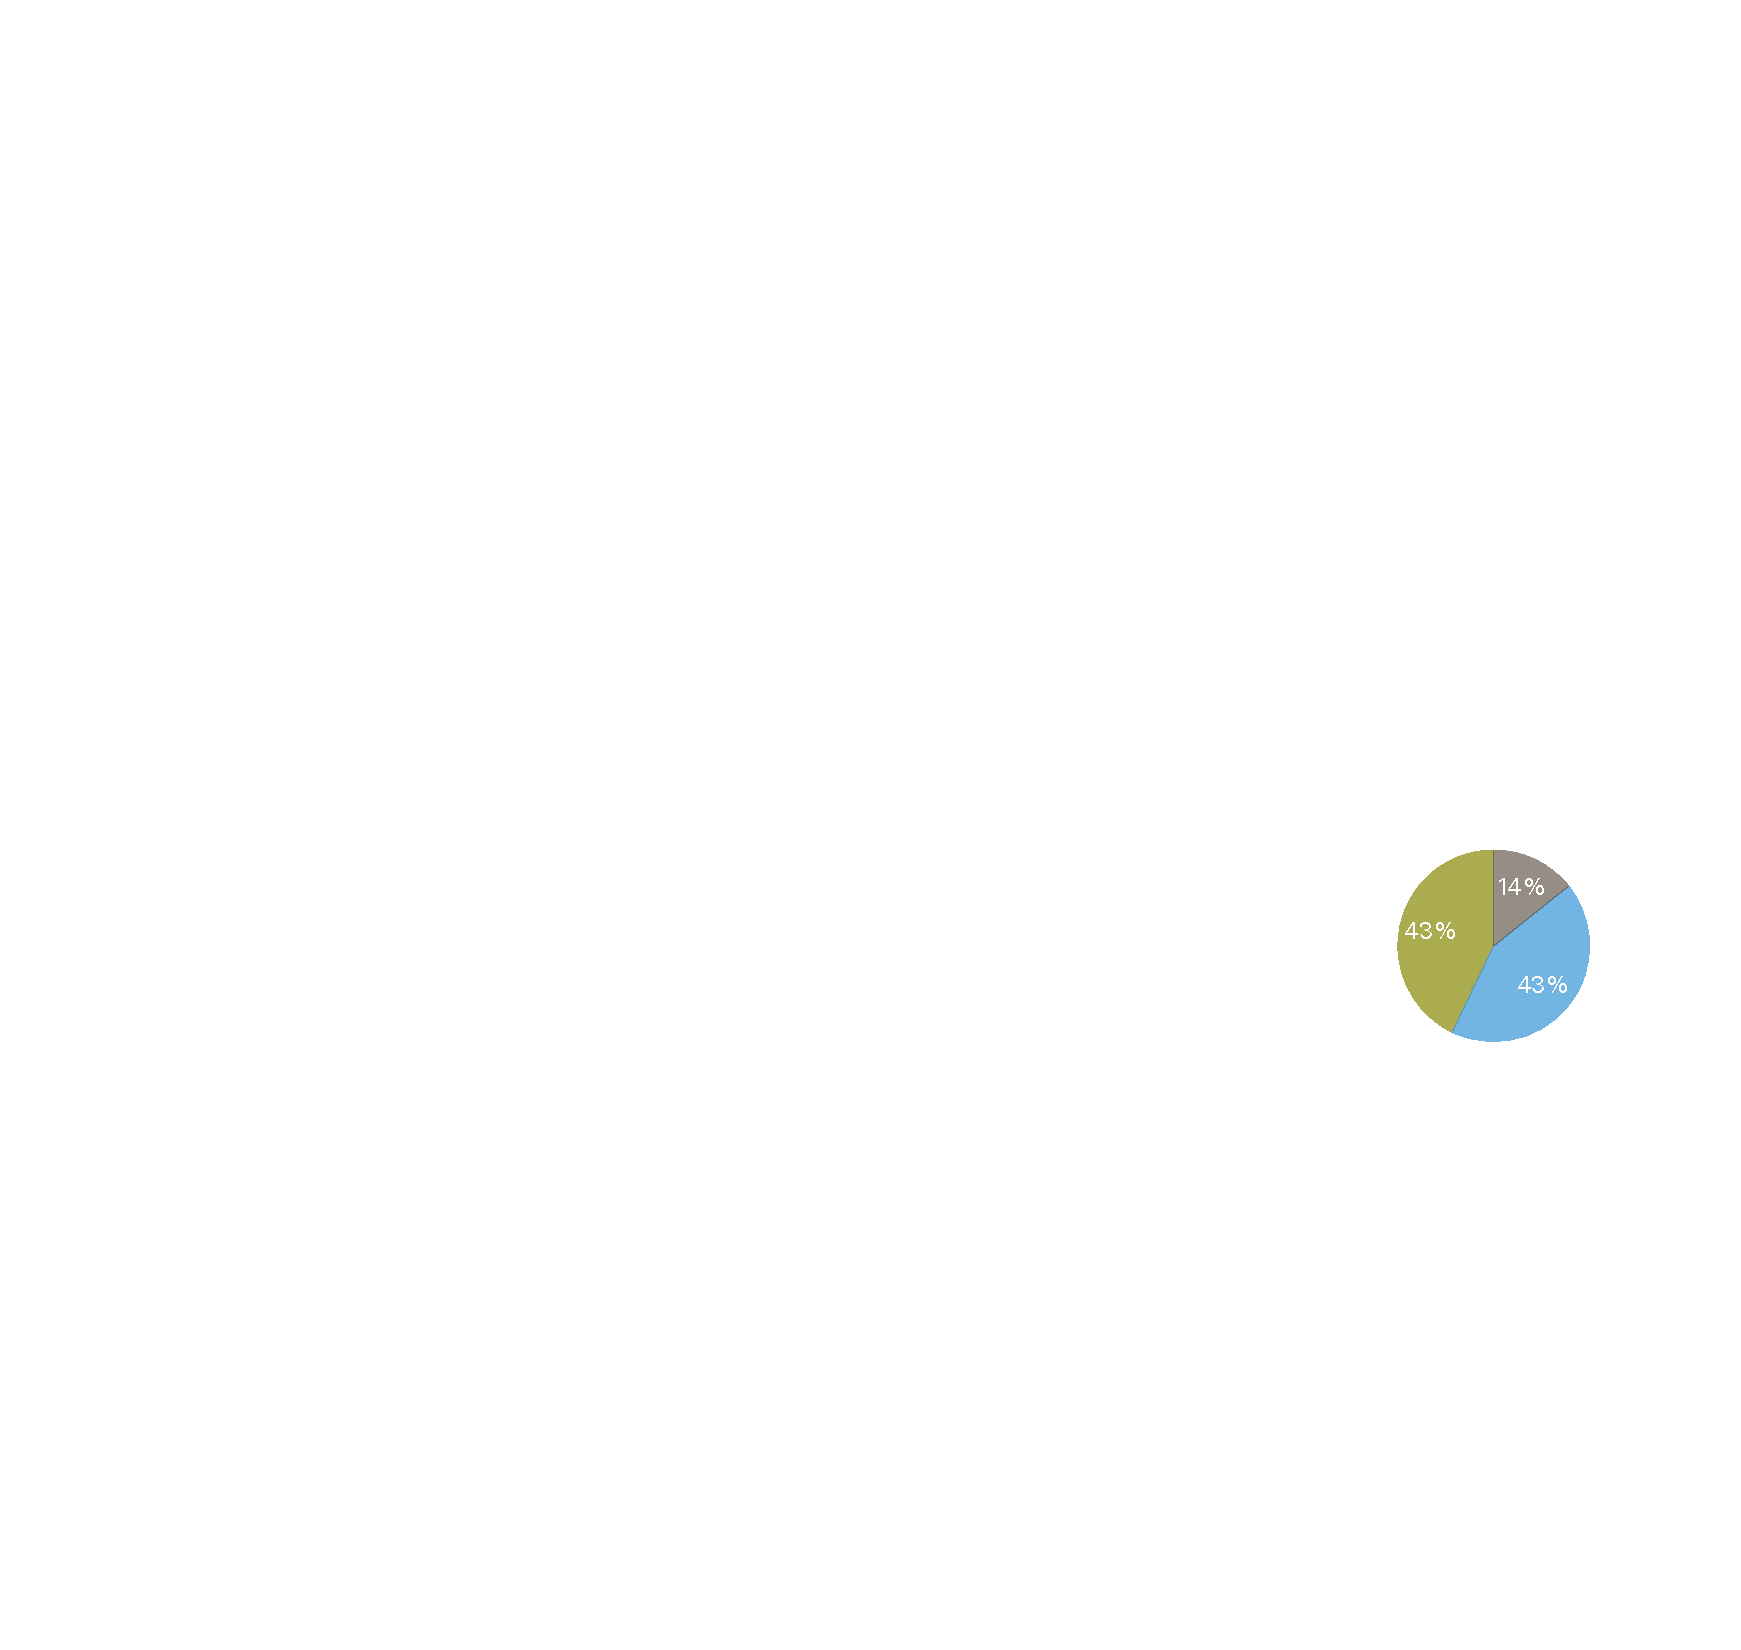
\includegraphics[scale=\graphicsscale]{resources/used-tools-charts-f}
        \caption{Whiteboard}
        \label{fig:used-tools-charts-f}
    \end{subfigure}
\end{minipage}
\caption{Auswertung der Verwendung von Tools zum Erstellen von Diagrammen}
\label{fig:used-tools-charts}
\end{figure}

Laut der Angaben der Teilnehmer konnten die Aufgaben in allen Fällen erfolgreich erfüllt werden (siehe Abbildung \ref{fig:evaluation-charts-a}). Weiterhin wurden die Aufgaben als nicht anstrengend eingeschätzt (siehe Abbildung \ref{fig:evaluation-charts-b}). Dies deutet darauf hin, dass für die Nutzerstudie angemessene Aufgaben gewählt wurden.

Obwohl es eine Einführung zu dem Prototypen gab (siehe Abschnitt \ref{subsec:user-study-setup}), wurden die Teilnehmer gefragt, ob sie die Aufgaben auch ohne diese Einführung erledigen könnten. Dies wurde zum großen Teil bestätigt, dennoch waren die Ergebnisse nicht ganz eindeutig (siehe Abbildung \ref{fig:evaluation-charts-c}). Bei der Vorbereitung des Aufbaus wurde überlegt, die Einführung wegzulassen. Da es sich aber bei den Softwaremodellierungswerkzeugen um ein Szenario handelt, in dem in der Regel das Anlernen der Bedienung und der Funktionen notwendig ist, wurde die Variante mit der Einführung bevorzugt.

\begin{figure}[!ht]

\newcommand{\legendscale}{0.9}
\newcommand{\subfigurewidth}{0.2\linewidth}
\newcommand{\graphicsscale}{0.75}    
\centering

% legend
\begin{subfigure}[t]{\textwidth}
    \centering
    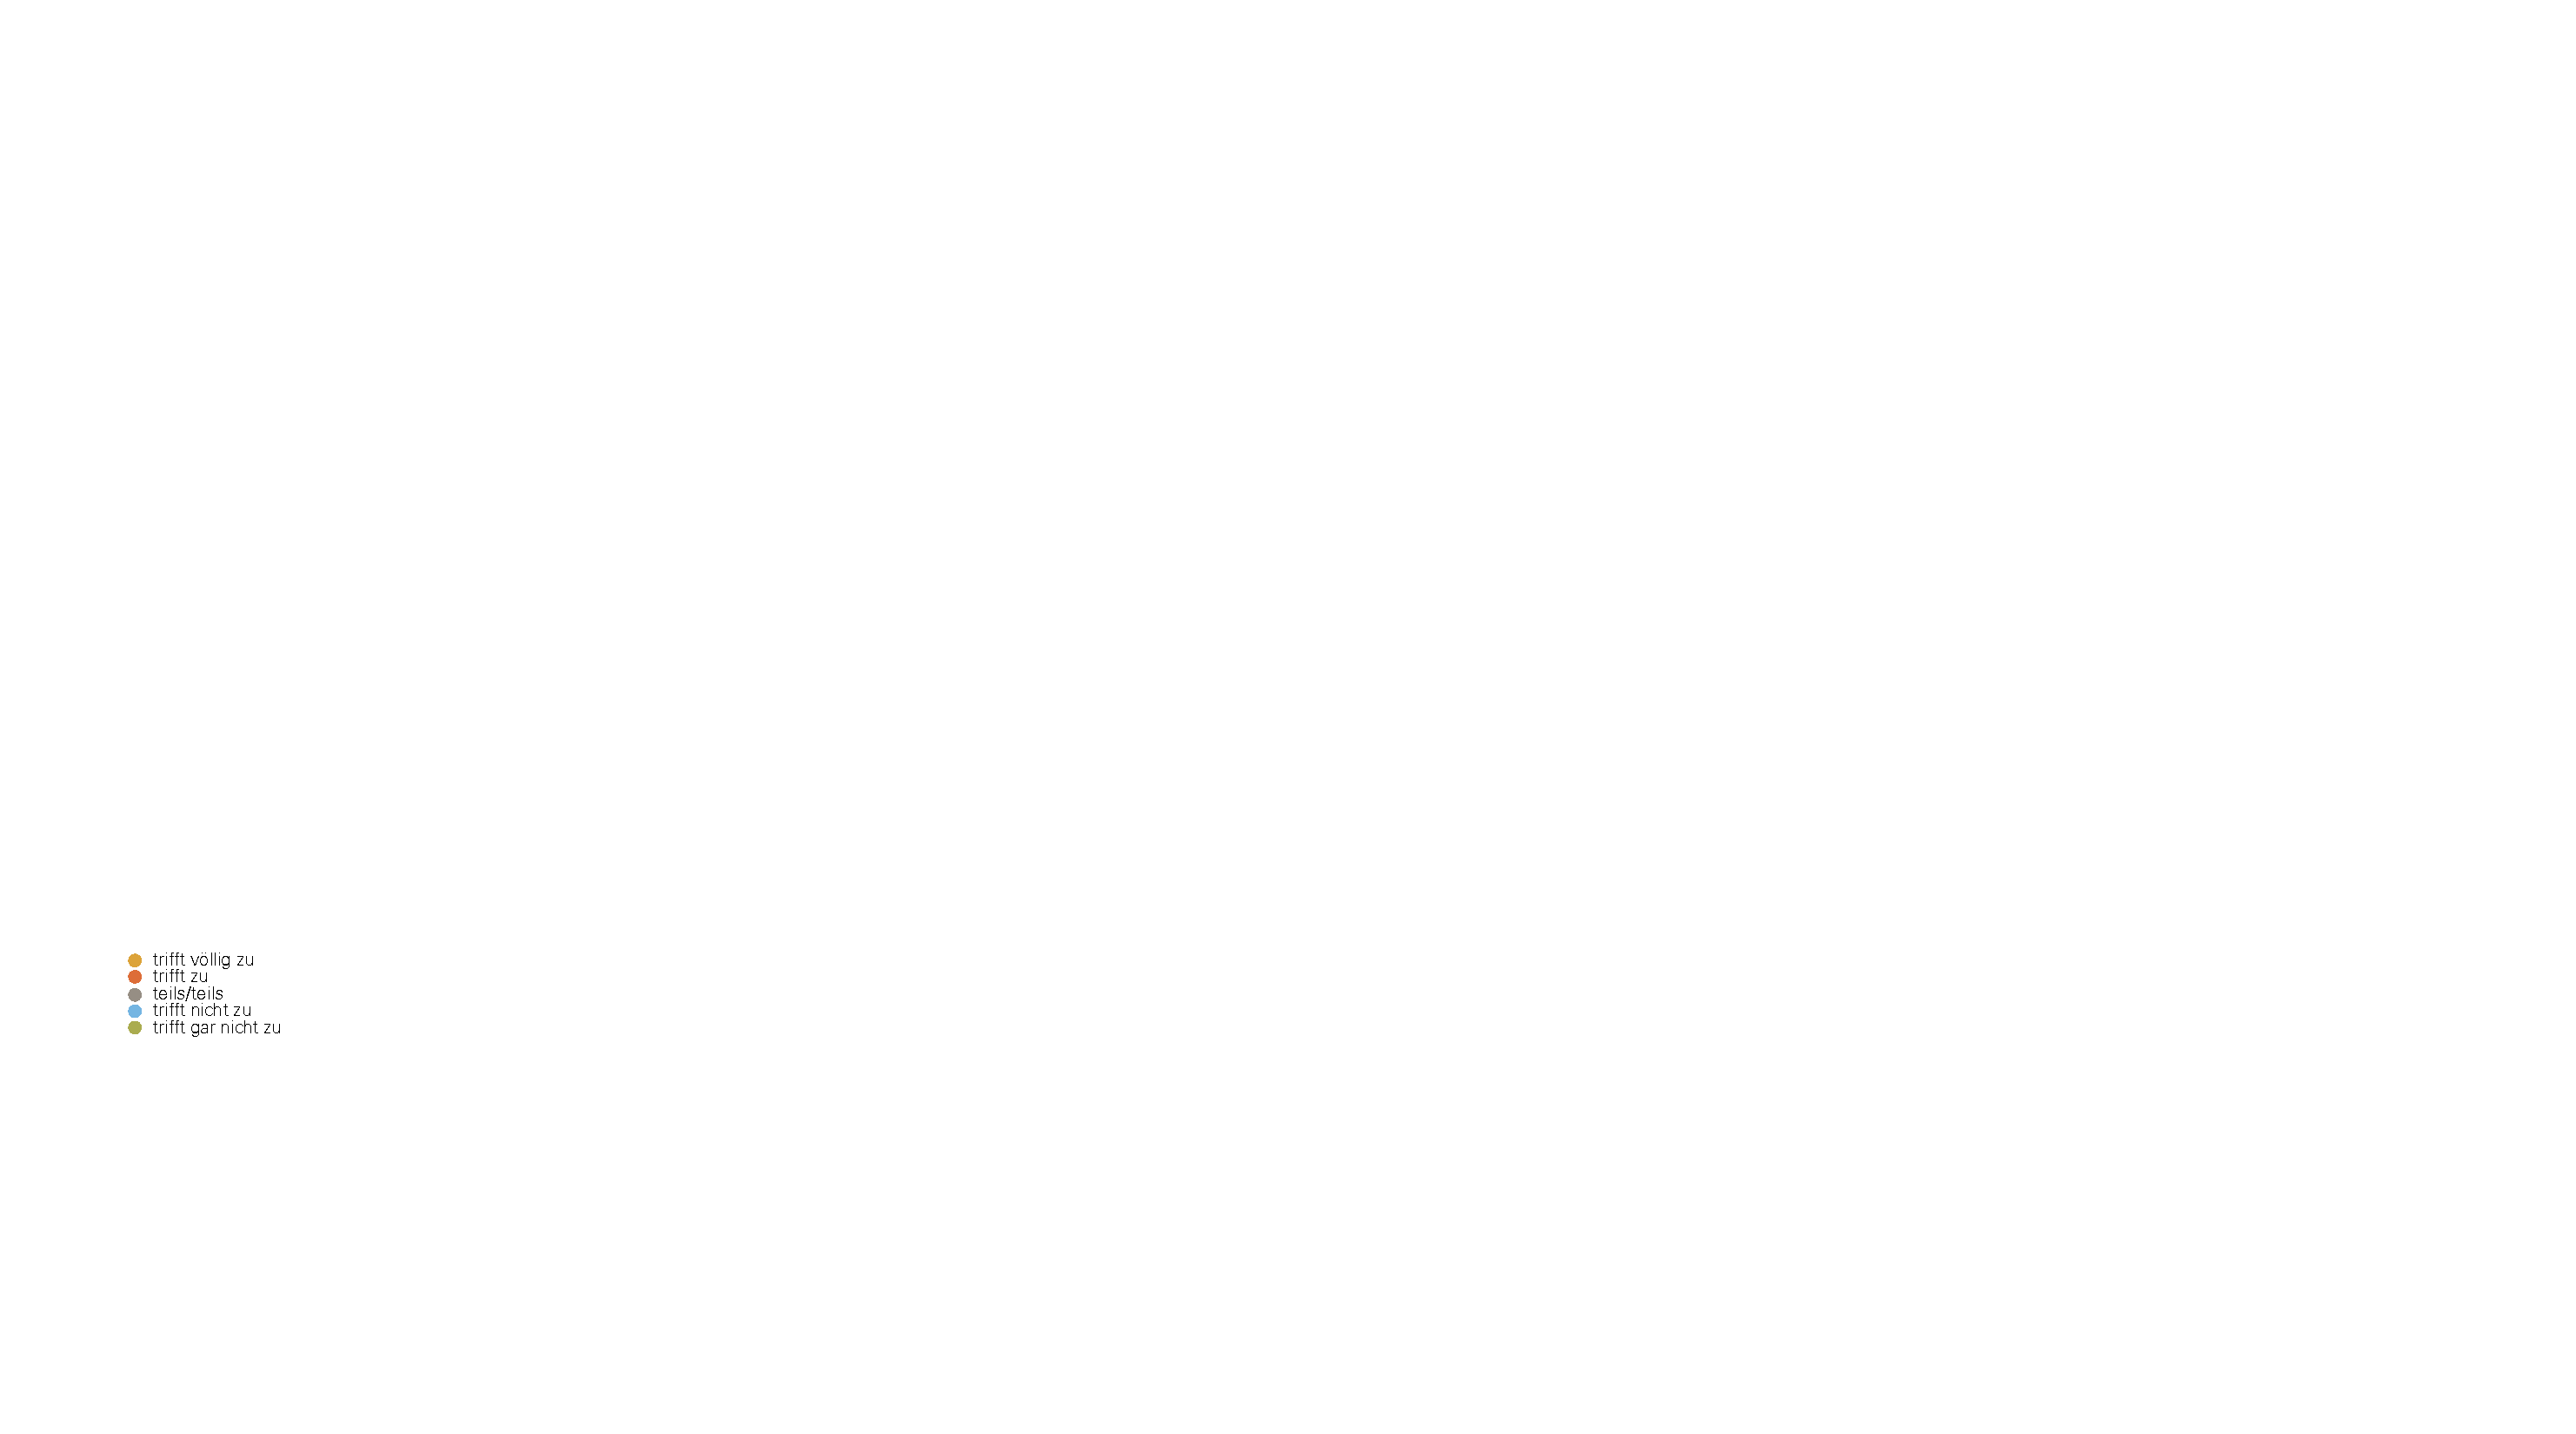
\includegraphics[scale=\legendscale]{resources/evaluation-charts-legend}
    \vspace{0.5cm}
\end{subfigure}

% charts
\foreach \i in {a,...,l}{%
\begin{subfigure}[t]{\subfigurewidth}
    \centering
    \includegraphics[scale=\graphicsscale]{resources/evaluation-charts-\i}
    \caption{}
    \label{fig:evaluation-charts-\i}
\end{subfigure}
}

% caption
\newcommand{\captionvalue}{Bewertung der Aussagen bzgl. der Evaluation des Konzepts}
\caption[\captionvalue]{
\captionvalue
\\\hspace{\textwidth}
\subref{fig:evaluation-charts-a} Ich habe meiner Meinung nach alle Aufgaben erfolgreich erfüllt.
\\\hspace{\textwidth}
\subref{fig:evaluation-charts-b} Die Erfüllung der Aufgaben war anstrengend.
\\\hspace{\textwidth}
\subref{fig:evaluation-charts-c} Ich denke, dass ich die Aufgaben auch ohne vorherige Vorstellung der möglichen Aktionen des Prototyps problemlos lösen könnte.
\\\hspace{\textwidth}
\subref{fig:evaluation-charts-d} Ich hatte das Programm die ganze Zeit unter Kontrolle.
\\\hspace{\textwidth}
\subref{fig:evaluation-charts-e} Die auf \enquote{Drag and Drop} basierende Verschiebungsaktion war verständlich.
\\\hspace{\textwidth}
\subref{fig:evaluation-charts-f} Durch die Einschränkung der freien Positionierung wurde der Aufwand an der Erstellung des Layouts reduziert.
\\\hspace{\textwidth}
\subref{fig:evaluation-charts-g} Die Einschränkung der freien Positionierung fand ich irritierend.
\\\hspace{\textwidth}
\subref{fig:evaluation-charts-h} Für mich war jederzeit erkennbar, an welche Stelle ich die angeklickte Klasse verschieben kann.
\\\hspace{\textwidth}
\subref{fig:evaluation-charts-i} Die automatischen Layout-Updates haben mich in der Erstellung des Diagramms gehindert.
\\\hspace{\textwidth}
\subref{fig:evaluation-charts-j} Das Layout der modellierten Diagramme fand ich ästhetisch ansprechend.
\\\hspace{\textwidth}
\subref{fig:evaluation-charts-k} Ich konnte Fehler, die während der Erfüllung der Aufgaben gemacht wurden, korrigieren.
\\\hspace{\textwidth}
\subref{fig:evaluation-charts-l} Ich bin der Meinung, dass ich die Aufgaben in einer Software ohne Layout-Unterstützung schneller erledigen könnte.
}
\label{fig:evaluation-charts}

\end{figure}

Da das umgesetzte Konzept viele neue Interaktionsparadigmen einsetzt, hat die Interaktion einen wesentlichen Teil der Bewertung gebildet. Dadurch wurde ermöglicht, die Erfüllung des Kriteriums der Benutzerfreundlichkeit zu beurteilen (siehe Abschnitt \ref{eval:user-friendly}).

Mehr als die Hälfte der Teilnehmer waren der Meinung, dass sie den Prototyp während der Erfüllung der Aufgaben unter Kontrolle hatten (siehe Abbildung \ref{fig:evaluation-charts-d}). Weiterhin konnte beobachtet werden, dass der in Abschnitt \ref{subsec:temporary-layer-mechanism} vorgestellte Mechanismus der temporären Schicht bzw. vereinfacht die auf \enquote{Drag and Drop} basierende Verschiebungsaktion von den Teilnehmern als intuitiv angesehen wurde. Dies wurde auch durch eine überwiegende Zustimmung im Fragebogen bestätigt (siehe Abbildung \ref{fig:evaluation-charts-e}).

Da der umgesetzte Ansatz keine freie Positionierung bietet, die von Werkzeugen die ausschließlich das manuelle Layout unterstützen (siehe Abschnitt \ref{sec:manual-layout}) bekannt ist, war die Einschränkung der freien Positionierung der Gegenstand der weiteren Bewertung. Die Mehrheit der Teilnehmer hat angegeben, dass die Einschränkung der freien Positionierung den Aufwand an der Erstellung des Layouts reduziert (siehe Abbildung \ref{fig:evaluation-charts-f}). Bis auf eine Ausnahme wurden die Teilnehmer durch diesen ungewöhnlicher Aspekt der Interaktion nicht verwirrt (siehe Abbildung \ref{fig:evaluation-charts-g}). Diese Resultate beweisen, dass die Einschränkung der freien Positionierung kein Problem dargestellt hat. An dieser Stelle ist allerdings auf die Vereinfachung der gewählten Aufgaben hinzuweisen. Um eine objektive Aussage über die Eignung dieses Verhaltens zu gewinnen, müsste das Konzept für einen allgemeineren Fall erweitert werden, z.B. durch die vollständige Unterstützung der Klassendiagramme.

Infolge des Einsatzes des baumbasierten Layouts hatte die Verschiebungsaktion zwei Funktionen. Einerseits konnte eine gesamte Vererbungshierarchie durch das Ziehen der Wurzelklasse verschoben werden. Anderseits konnte die Reihenfolge der Geschwisterklassen mit Hilfe der Verschiebungsaktion variiert werden. Obwohl die möglichen Zielpositionen der Verschiebung zum großen Teil für die Teilnehmer erkennbar waren (siehe Abbildung \ref{fig:evaluation-charts-h}), sind die Ergebnisse nicht überzeugend. Deshalb sollte insbesondere in einer allgemeinen Version des Algorithmus über eine potentielle Visualisierung der Verschiebungsoptionen nachgedacht werden.

Die automatischen Layout-Updates haben keine Hinderung in der Erstellung des Diagramms dargestellt (siehe Abbildung \ref{fig:evaluation-charts-i}). Dagegen wurde die Ästhetik des Layouts größtenteils als ansprechend empfunden (siehe Abbildung \ref{fig:evaluation-charts-j}). Die möglichen Ursachen für eine nicht überzeugende Zustimmung sind auf die Überlappung der Pfeilspitzen bei der Vererbungsrelationen und die Umbrüche der Klassennamen zurückzuführen.

Die Antworten bzgl. der Möglichkeit der Fehlerkorrektur während der Erfüllung der Aufgaben unterscheiden sich erheblich (siehe Abbildung \ref{fig:evaluation-charts-k}). Der Grund dafür war eine unterschiedliche Fehlerquote der einzelnen Teilnehmer. Wenn ein Fehler gemacht wurde, der mit Hilfe der im Prototyp verfügbaren Aktionen nicht korrigiert werden konnte, musste die Aufgabe wiederholt werden. Die fehlenden Aktionen werden im Folgenden diskutiert. Trotz der Unvollständigkeit des Prototyps waren die Teilnehmer vorwiegend der Meinung, dass die Layout-Unterstützung ein Zeitersparnis im Vergleich zu anderen Werkzeugen bringt (siehe Abbildung \ref{fig:evaluation-charts-l}). Dadurch wurde der geschaffene Mehrwert des Ansatzes gezeigt.

Wie bereits in Kapitel \ref{chapter:prototype} erwähnt wurde, ist der umgesetzte Prototyp nicht ausgereift und unterstützt viele Funktionen nicht. Die fehlenden Funktionen bilden den Gegenstand für einen weiteren Teil der Nutzerstudie. Einerseits wurde beobachtet, welche nicht implementierten Funktionen die Teilnehmer auszuführen versucht haben. Anderseits wurden die Teilnehmer explizit nach den vermissten Funktionen gefragt. Die Ergebnisse sind in Abbildung \ref{fig:missed-prototype-functions} visualisiert.

\begin{figure}[hbt]
    \centering
    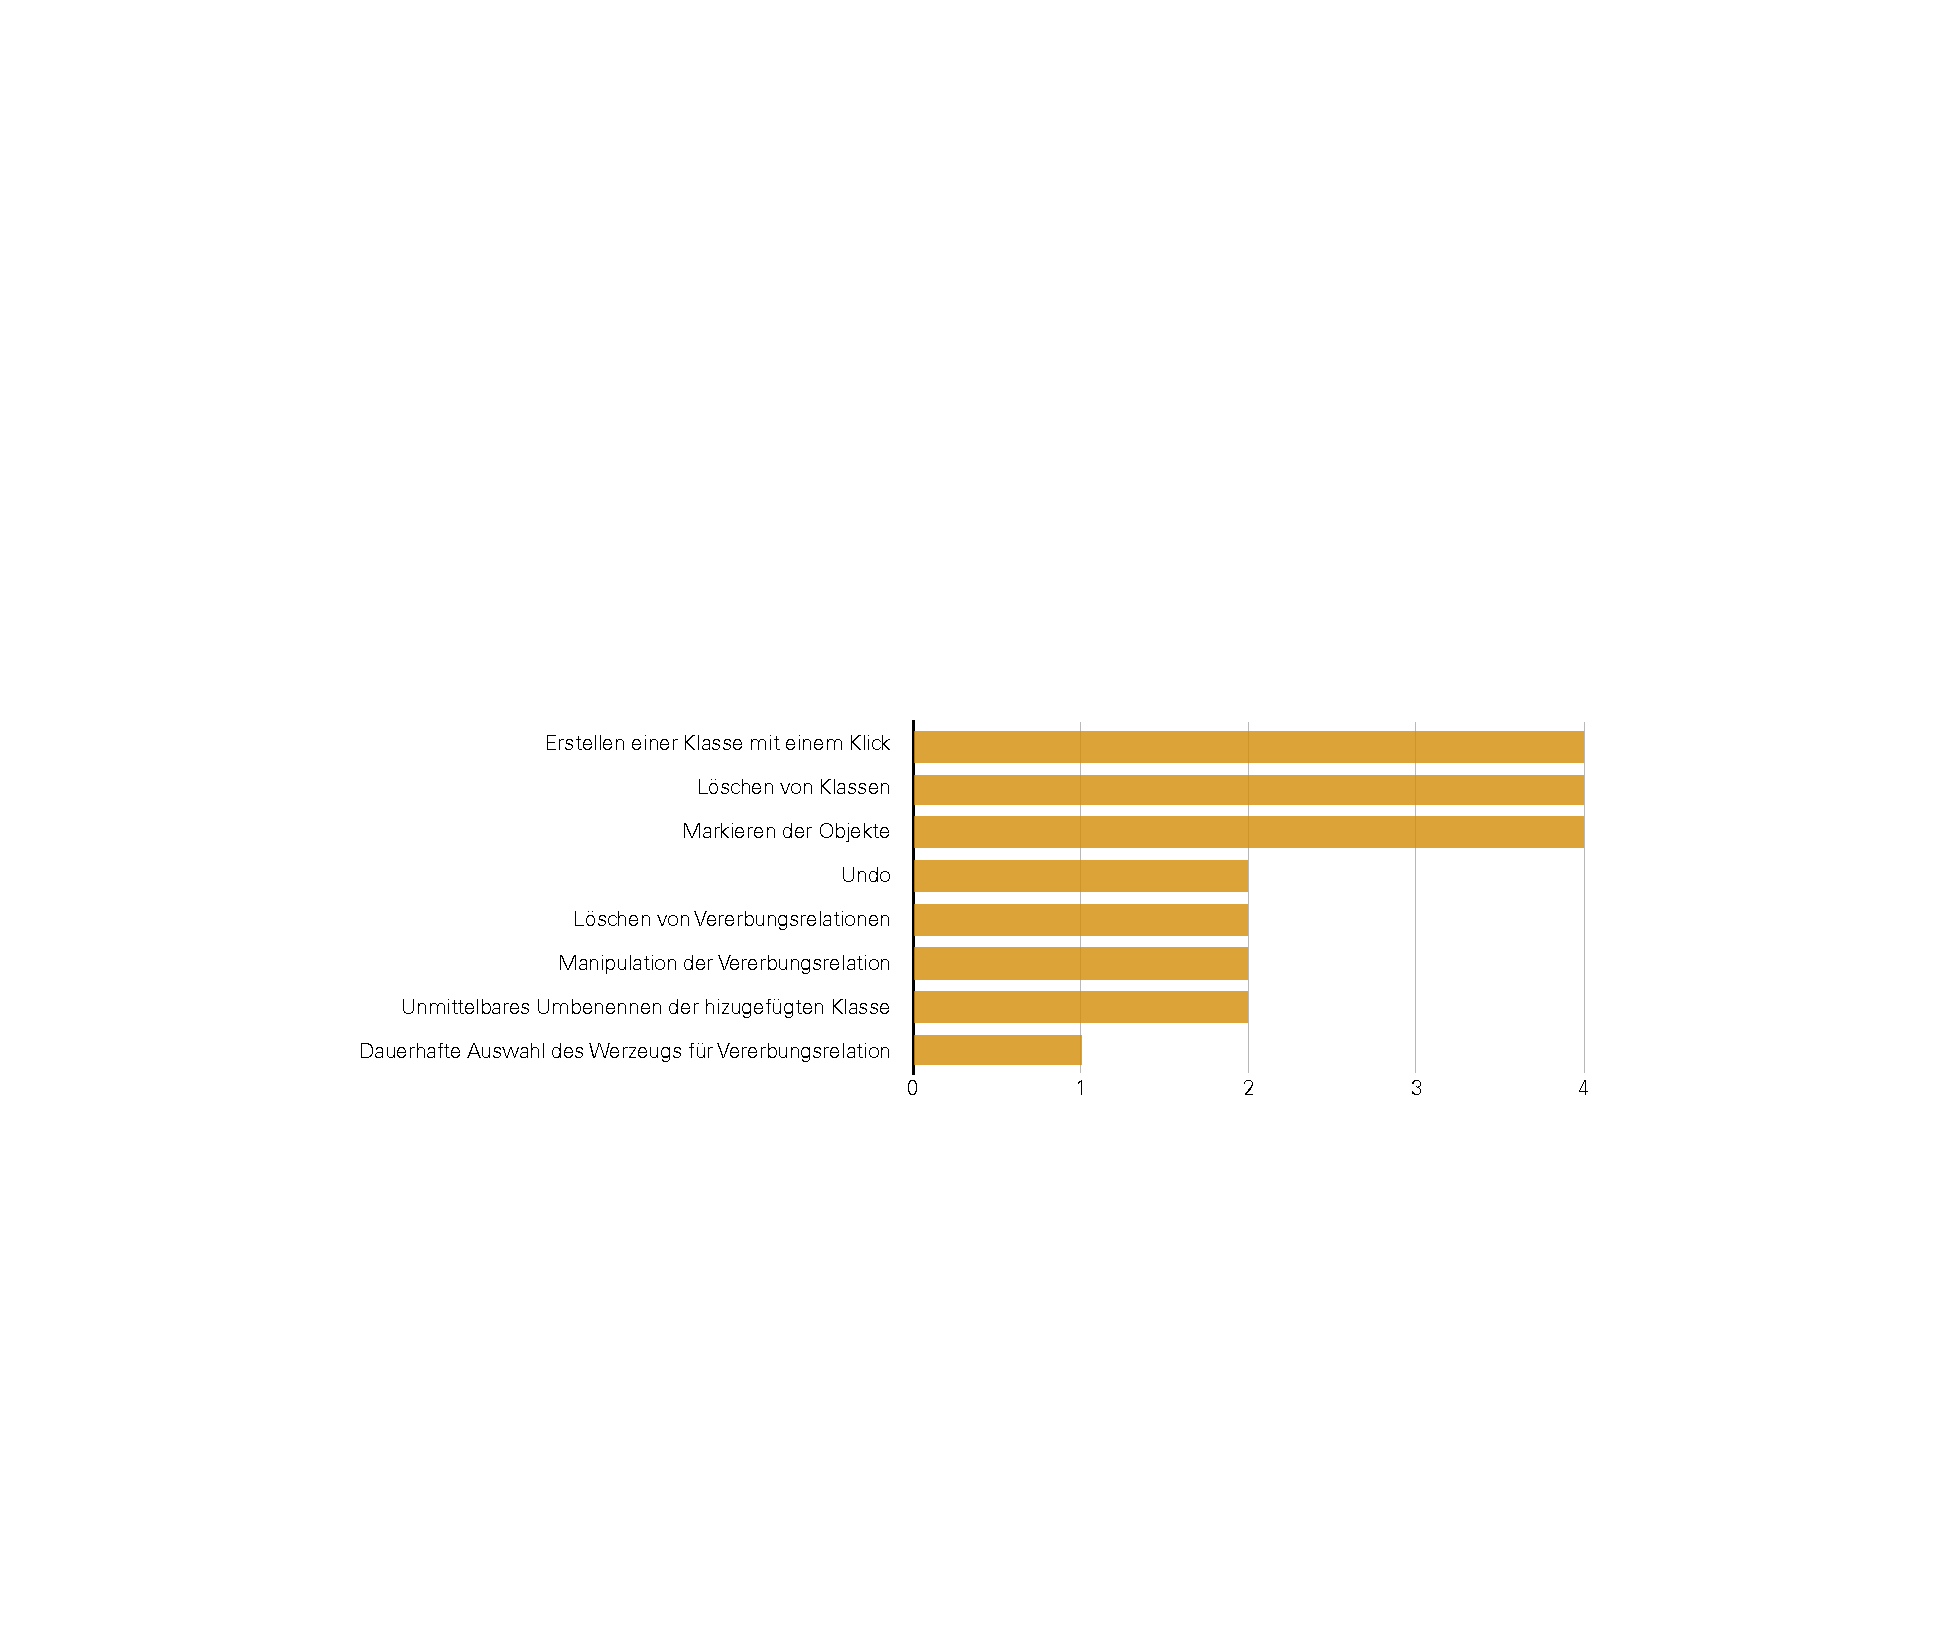
\includegraphics[width=\textwidth]{resources/missed-prototype-functions}
    \caption{Übersicht der vermissten Funktionen im Prototyp}
    \label{fig:missed-prototype-functions}
\end{figure}

Als eine der meist vermissten Funktionen gilt die Möglichkeit des Hinzufügens einer neuen Klasse mit einem Klick bzw. Doppelklick auf das Icon in der Sidebar. Die Einschränkung auf das \enquote{Drag and Drop} wurde als ungenügend eingeschätzt, insbesondere wenn mehrere Klassen auf einmal hinzugefügt werden sollten. Die Behebung dieser Schwachstelle besteht darin, beide Techniken zu unterstützen und bei dem Klick, die neue Klasse an eine vorgegebene Position im Diagramm zu platzieren.

Um die Korrektur von Fehlern zu ermöglichen, müssten Funktionen wie Löschen von Objekten, Manipulation der Vererbungsrelationen und \enquote{Undo} zur Verfügung stehen. Für die objektbezogenen Objekte ist weiterhin die Funktion deren Markierung im Canvas notwendig, die auch für eine gleichzeitige Verschiebung von mehreren Klassen eingesetzt wurde. Die genannten Funktionen bilden eine Gruppe von Standardfunktionen, die in der Regel in einer kompletten Anwendung unterstützt werden sollten und durch die Teilnehmer der Nutzerstudie vermisst wurden. Deren Implementierung im Prototyp für Zwecke dieser Arbeit wurde aus zeitlichen Gründen weggelassen. Dennoch werden alle genannten Funktionen im Konzept berücksichtigt, denn sie können mit Hilfe von Layout-Ereignissen beschrieben werden (siehe Abschnitte \ref{sec:layout-calculation} und \ref{subsubsec:component-events}).

Die Abbildung \ref{fig:missed-prototype-functions} zeigt weiterhin zwei kleinere Probleme der Benutzeroberfläche im Prototyp. In zwei Fällen fänden die Teilnehmer intuitiver, wenn neu hinzugefügten Klassen den Fokus behalten würden, um den Klassennamen auch ohne einen zusätzlichen Doppelklick eingeben zu können. Des Weiteren wurde in einem Fall angemerkt, dass das Werkzeug für die Vererbungsrelation dauerhaft ausgewählt werden könnte. Aufgrund der Kompliziertheit mit einer ständigen Auswahl des Icons in der Sidebar hat die Mehrheit der Teilnehmer zu der Alternative mit der Taste \texttt{CTRL} (siehe Abschnitt \ref{subsec:supported-actions}) gewechselt. Beide Probleme könnten durch einfache Anpassungen im Prototyp behoben werden und haben keinen Einfluss auf das gesamte Konzept. Das Erstellen von Relationen könnte zusätzlich noch mit an die Klassen gebundenen Buttons wie in \textit{Visual Paradigm} durchgeführt werden \cite{14Visual}. Insbesondere würde dies ein angemerktes Problem mit der nicht intuitiven Positionierung von neu hinzugefügten Klassen lösen.

Der Ablauf der Modellierung hat sich je nach dem Teilnehmer und der konkreten Aufgabe unterschieden. Im Wesentlichen wurden die Klassen nacheinander hinzugefügt und jede Klasse direkt umbenannt und in eine Vererbungshierarchie eingeordnet. In einigen Fällen wurde versucht, die Klassen frei zu positionieren. Die Funktionsweise wurde den Teilnehmern vor allem durch das Platzhalter-Objekt sichtbar gemacht und sie haben sich an die Einschränkung der freien Positionierung und das halbautomatische Layout angewöhnt. Ferner wurde die Zentrierung des Inhalts bei der Vergrößerung des Fensters als natürlich empfunden.

Die Nutzerstudie hat bestätigt, dass der entwickelte Ansatz den Prozess der Layout-Erstellung deutlich vereinfacht. Obwohl der umgesetzte Prototyp sehr eingeschränkt war und nur die Modellierung von einfachen Aufgaben ermöglicht hat, haben sich die Möglichkeiten der Interaktion dank der eingesetzten Bedienungskonzepten als intuitiv aufgewiesen. Weiterhin wurden durch die Nutzerstudie Stellen entdeckt, die verbessert bzw. erweitern werden könnten. Die gewonnenen Informationen sind für eine weitere Entwicklung des Prototyps und vor allem des zu Grunde liegenden Ansatzes sehr hilfreich.

\section{Erfüllung der Kriterien}
\label{sec:criteria-evaluation}

Im Folgenden werden die Kriterien aus Abschnitt \ref{sec:criteria} einzeln aufgegriffen und deren Erfüllung in dem entwickelten Ansatz kritisch u.a. anhand von Ergebnissen der Nutzerstudie bewertet:

\begin{enumerate}[label={K.\arabic*}]

\item
\label{eval:gui}
\textbf{GUI}
Die Bearbeitung des Diagramms basiert auf Mechanismen, die für klassische grafische Benutzeroberflächen ausgelegt sind. Insbesondere ist der Einsatz des Mauszeigers von Bedeutung, wodurch eine sequenzielle Ausführung von Bearbeitungsaktionen ermöglicht wird. Somit hält sich der Ansatz an den Rahmenbedingungen aus Abschnitt \ref{sec:thesis-conditions} und erfüllt das Kriterium \ref{req:gui}.

\item
\label{eval:interactivity}
\textbf{Interaktivität}
Das modellierte Diagramm wird in einem Canvas dargestellt, worin es unmittelbar bearbeitet werden kann. Die Grundlage dafür bilden die Bearbeitungsaktionen (siehe Abschnitt \ref{subsec:edit-actions}), die durch den Nutzer ausgeführt werden. Während bzw. nach der Ausführung einer Bearbeitungsaktion reagiert das System, indem das Layout des Diagramms mit Hilfe von Layout-Übergängen (siehe Abschnitt \ref{subsec:layout-transitions}) angepasst wird. Dadurch dass der Prozess der Diagramm-Bearbeitung als eine Sequenz von Bearbeitungsaktionen aufgefasst werden kann, ist die Interaktivität in dem Ansatz fest verankert. Das Kriterium \ref{req:interactivity} wird daher ebenfalls erfüllt.

\item
\label{eval:immediate-feedback}
\textbf{Unmittelbares Feedback}
Wie in Abschnitt \ref{subsec:temporary-layer-mechanism} erläutert wurde, macht sich die Verschiebungsaktion den neu eingeführten Mechanismus der temporären Schicht zunutze. Während der Verschiebung wird das Layout des Diagramms kontinuierlich angepasst, wobei die Änderung anhand eines Platzhalters für den verschobenen Knoten und einer Animation des Layout-Übergangs visualisiert wird. Dem Nutzer wird im Verlauf der Aktion ständig das Ergebnis präsentiert, wodurch eine unmittelbare Feedback-Schleife erreicht wird (Kriterium \ref{req:immediate-feedback}). Da alle anderen unterstützten Bearbeitungsaktionen diskret sind, setzen sie das unmittelbare Feedback nicht ein. Dagegen wird erst nach ihrer Ausführung der Layout-Übergang initiiert. Die Funktionsweise von beiden Arten der Bearbeitungsaktionen hat sich in der Nutzerstudie als verständlich aufgewiesen (siehe Abschnitt \ref{subsec:user-study-evaluation}).

\item
\label{eval:editing-support}
\textbf{Förderung des Prozesses der Diagramm-Erstellung}
Die inkrementelle Bearbeitung der Diagramme bildet eine Grundlage des präsentierten Ansatzes. Sie erfolgt durch die Ausführung von Bearbeitungsaktionen, die entweder den Inhalt oder das Layout des Diagramms modifizieren (siehe Abschnitt \ref{subsec:edit-actions}). Die Änderung des Inhalts bewirkt eine automatische Anpassung des Layouts, welches wiederum durch den Nutzer mit Hilfe der Verschiebungsaktion in einem beschränkten Maß nach seinen Präferenzen verändert werden kann. Durch die fehlende Möglichkeit der expliziten Anpassung von Layout-Eigenschaften\footnote{Insbesondere handelt es sich an dieser Stelle um die Einschränkung der freien Positionierung.} kann sich der Nutzer in der Bearbeitung des Diagramms gehindert fühlen. Dies wurde in der Nutzerstudie untersucht und für das gewählte Beispiel hat dies kein Problem dargestellt, wodurch das Kriterium \ref{req:editing-support} erfüllt wird. Eine derartige Eignung für allgemeinere Fälle wird in Abschnitt \ref{subsec:user-study-evaluation} diskutiert.

\newpage

\item
\label{eval:mental-map}
\textbf{Erhaltung des mentalen Modells}
Wie in Kapitel \ref{chapter:interactive-approach} erläutert wurde, werden während der Bearbeitung des Diagramms Layout-Änderungen berechnet und auf das Diagramm angewendet. Dabei wird es angestrebt, sie minimal zu halten. Des Weiteren werden die Layout-Änderungen in sequenzielle Layout-Übergänge gekapselt (siehe Abschnitt \ref{subsec:layout-transitions}), wodurch eine getrennte Wahrnehmung durch den Nutzer erreicht wird. Zudem werden die Layout-Übergänge animiert, so dass die neuen Positionen der Objekte ermittelt werden können. Diese Maßnahmen sorgen für die Erhaltung des mentalen Modells (Kriterium \ref{req:mental-map}).

\item
\label{eval:focus-on-the-content}
\textbf{Förderung der Konzentration auf den Inhalt}
Durch die automatische Layout-Berechnung und die Einschränkung der Möglichkeiten an der manuellen Layout-Anpassung wird der Aufwand an der Erzeugung des Layouts verringert, was durch die Nutzerstudie bestätigt wurde (siehe Abschnitt \ref{subsec:user-study-evaluation}). Dies führt dazu, dass sich der Nutzer in erster Linie mit der Erstellung des Inhalts auseinandersetzt und das berechnete Layout nur ein wenig variieren kann. Damit wird das Kriterium \ref{req:focus-on-the-content} für das gewählte Beispiel erfüllt. Allerdings ist es zu erwähnen, dass eine Verallgemeinerung des Konzeptes für eine vollständige visuelle Sprache (z.B. für Klassendiagramme) die Notwendigkeit der Unterstützung von weiteren manuellen Layout-Anpassungen mit sich bringen kann.

\item
\label{eval:aesthetics-criteria}
\textbf{Berücksichtigung der ästhetischen Prinzipien}
Die ästhetischen Prinzipien aus Abschnitt \ref{sec:aesthetics-criteria} werden in dem entwickelten Ansatz durch den Algorithmus der Layout-Engine (siehe Abschnitt \ref{sec:layout-calculation}) und den Einsatz der Layout-Patterns (siehe Abschnitt \ref{sec:layout-patterns}) umgesetzt. Dadurch dass die unterstützte Notation der Klassendiagramme eingeschränkt wurde, konnte die Berücksichtigung der ästhetischen Prinzipien in dem Algorithmus für das baumbasierte Layout \ref{subsubsec:tree-layout-algorithm} deutlich vereinfacht werden. Im Folgenden wird gezeigt, inwiefern das Kriterium \ref{req:aesthetics-criteria} erfüllt wurde, indem auf die einzelnen ästhetischen Prinzipien eingegangen wird.

Durch die baumbasierte Struktur und die Umsetzung des impliziten Layout-Patterns für die Verhinderung der Knoten-Überlappung (siehe Abschnitt \ref{subsubsec:prevention-of-node-overlap}) wird sichergestellt, dass sich die Klassen nicht überlappen und entsprechend voneinander entfernt sind (Prinzip \ref{pri:distances}). Die Verbindung der Klassen erfolgt ausschließlich durch die Erstellung von azyklischen Vererbungsrelationen, wodurch die Kantenkreuzungen komplett ausgeschlossen werden (Prinzip \ref{pri:edge-crossings}). Obwohl der Ansatz für die Unterstützung der \enquote{Gabelform} für Vererbungsrelationen ausgelegt ist, wurde diese aus zeitlichen Gründen im Prototyp nicht umgesetzt. Dahingegen wurde eine direkte Verbindung gewählt (Prinzip \ref{pri:inheritance-relation}). Da die Vererbung der einzige unterstützte Relationstyp ist und die Relationen durch direkte Verbindungen dargestellt werden, sind die Prinzipien \ref{pri:edge-bends} und \ref{pri:orthogonality} für das Beispiel überflüssig und wurden nicht betrachtet. Die hierarchischen Kanten der Vererbung werden aufgrund der Baumstruktur des Diagramm in einem vertikalen Verlauf dargestellt (Prinzip \ref{pri:edge-direction}). Somit können Vererbungshierarchien mit mehreren Ebenen gebildet werden, die sich nach dem Prinzip der Darstellung von Hierarchien richten (Prinzip \ref{pri:hierarchies}) und für die Positionierung der Klassen Symmetrie einsetzten (Prinzip \ref{pri:symmetry}).

\newpage

Die einzelnen Vererbungshierarchien werden kompakt in einer horizontalen Linie im Diagramm angeordnet (Prinzip \ref{pri:related-elements-placement}). Auf dieser Weise werden ebenso die nicht verbundenen Klassen dargestellt. Durch den Nutzer kann ihre Reihenfolge geändert werden, so dass sie auch am Rand des Diagramms positioniert werden können (Prinzip \ref{pri:unconnencted-elements-placement}). Um den Canvas möglichst optimal auszunutzen und das Prinzip \ref{pri:drawing-area} einzuhalten, wird ein großer Wert auf die Verteilung der Objekte gelegt, u.a. durch die automatische Zentrierung des Diagramms (siehe Abschnitt \ref{subsubsec:centering-of-diagram-content}). Die horizontale Anordnung in dem Algorithmus für das baumbasierte Layout hat allerdings mit dem Problem der Skalierbarkeit zu kämpfen. Die Größe des Canvas im Prototyp ist durch die Größe des Fensters bestimmt und wird nicht erweitert, wenn der Inhalt des Diagramms nicht hineinpasst. Dies könnte durch den Einsatz eines \enquote{Scroll Views} gelöst werden. Durch mehrere vereinzelte Klassen oder Klassenhierarchien könnte trotzdem die Breite des Diagramms unangemessen zu der Höhe sein und dadurch das Prinzip \ref{pri:drawing-area} verletzen. In der Regel kommen in den Klassendiagrammen Klassen vor, die miteinander verbunden sind. Des Weiteren wird in \cite{Ambler02Agile} empfohlen, Klassendiagramme klein zu halten, so dass sie nur wenige Klassen beinhalten. Dadurch könnte das genannte Problem umgegangen werden. Für eine objektive Aussage wäre allerdings eine weitere Untersuchung notwendig.

\item
\label{eval:syntax-and-semantics}
\textbf{Berücksichtigung der Syntax und Semantik}
Der präsentierte Ansatz sieht es vor, die Layout-Berechnung anhand der Semantik der Objekte durchzuführen. Dadurch, dass sich das gewählte Beispiel auf stark vereinfachte Klassendiagramme beschränkt, wurde der Einfachheit halber kein Metamodell eingesetzt. Obwohl die Beschreibung der Syntax und Semantik in dem Ansatz nicht formalisiert ist, werden die Syntax- und Semantikregeln für Klassendiagramme in dem Algorithmus für das baumbasierte Layout eingehalten. Leider konnte der diagrammspezifische Aspekt des Ansatzes aus zeitlichen Gründen nicht tiefgründig ausgearbeitet werden und das Kriterium \ref{req:syntax-and-semantics} wurde nur teilweise erfüllt. Dahingegen wurde der Schwerpunkt der Arbeit auf die Interaktivität und die Gestaltung der Bedienungsmechanismen gelegt. An dieser Stelle bildet sich ein Potential für eine weitere Entwicklung, die in Abschnitt \ref{sec:outlook} thematisiert wird.

\item
\label{eval:user-friendly}
\textbf{Benutzerfreundlichkeit}
Die Benutzerfreundlichkeit der eingesetzten Bedienungsmechanismen wurde im Rahmen der Nutzerstudie untersucht. Die Auswertung der Ergebnisse wurde in Abschnitt \ref{subsec:user-study-evaluation} aufgeführt.

\end{enumerate}

% kleine Diagramme sind schnell zu zeichnen, manuelle Bearbeitung skaliert nicht mit der Größe des Diagramms \cite{Eichelberger05Aesthetics}

\section{Zusammenfassung}
\label{sec:evaluation-summary}
